% ==============================================================================
% RELATÓRIO TÉCNICO — PRÁTICA 3: PROJETO DE FILTRO FIR PASSA-BAIXA
% Centro Universitário SENAI CIMATEC — Processamento Digital de Sinais (2026)
% Professor: Elio Pithon Sarno Filho
%
% INSTRUÇÕES DE COMPILAÇÃO (LOCAL / OVERLEAF):
%   Compilador: pdfLaTeX. Mantenha os 8 arquivos .pdf de `figures/` em
%   `./figures/`, `../figures/` ou na mesma pasta deste `main.tex`.
% ==============================================================================
\documentclass[11pt,a4paper]{article}

% --- Codificação, Fontes e Idioma ---
\usepackage[utf8]{inputenc}
\usepackage[T1]{fontenc}
\usepackage[brazilian]{babel}
\usepackage{lmodern}
\usepackage{microtype}
\usepackage{indentfirst}

% --- Geometria, Espaçamento e Controle de Floats ---
\usepackage[a4paper, top=2.2cm, bottom=2.2cm, left=2.1cm, right=2.1cm, headheight=14.5pt]{geometry}
\linespread{1.10}
\setlength{\parskip}{3pt}
\usepackage{fancyhdr}
\usepackage{titlesec}
\usepackage{enumitem}
\usepackage{placeins}

\renewcommand{\topfraction}{0.90}
\renewcommand{\bottomfraction}{0.85}
\renewcommand{\textfraction}{0.08}
\renewcommand{\floatpagefraction}{0.80}
\setlength{\floatsep}{9pt plus 2pt minus 2pt}
\setlength{\textfloatsep}{11pt plus 2pt minus 2pt}
\setlength{\intextsep}{9pt plus 2pt minus 2pt}

% --- Matemática e Unidades ---
\usepackage{amsmath, amssymb, mathtools}
\usepackage{siunitx}
\sisetup{
    output-decimal-marker = {,},
    group-separator = {.},
    group-digits = integer,
    group-minimum-digits = 4,
    detect-all = true,
    per-mode = symbol
}

% --- Tabelas, Figuras e Cores ---
\usepackage{booktabs}
\usepackage{array}
\usepackage{tabularx}
\usepackage{adjustbox}
\usepackage[table]{xcolor}
\usepackage{graphicx}
\graphicspath{{./figures/}{../figures/}{./}}
\usepackage{float}
\usepackage{caption}
\captionsetup{
    font=small,
    labelfont=bf,
    labelsep=period,
    justification=justified,
    skip=5pt
}

% --- Diagramas Vetoriais (TikZ) ---
\usepackage{tikz}
\usetikzlibrary{arrows.meta, positioning, calc, shapes.geometric}

% --- Listagens de Código MATLAB ---
\usepackage{listings}

% Paleta institucional e de código
\definecolor{cimatecblue}{RGB}{0, 74, 143}
\definecolor{cimatecgray}{RGB}{242, 245, 249}
\definecolor{codebg}{RGB}{248, 249, 250}
\definecolor{codeframe}{RGB}{210, 215, 220}
\definecolor{codekw}{RGB}{0, 64, 150}
\definecolor{codecomment}{RGB}{34, 120, 55}
\definecolor{codestr}{RGB}{163, 21, 21}
\definecolor{rowpass}{RGB}{235, 248, 238}
\definecolor{rowfail}{RGB}{253, 242, 242}

\lstdefinestyle{matlabstyle}{
    language=Matlab,
    backgroundcolor=\color{codebg},
    frame=single,
    rulecolor=\color{codeframe},
    basicstyle=\ttfamily\footnotesize,
    keywordstyle=\color{codekw}\bfseries,
    commentstyle=\color{codecomment}\itshape,
    stringstyle=\color{codestr},
    numbers=left,
    numberstyle=\tiny\color{gray!80!black},
    stepnumber=1,
    numbersep=7pt,
    tabsize=4,
    showspaces=false,
    showstringspaces=false,
    breaklines=true,
    breakatwhitespace=true,
    captionpos=b,
    aboveskip=7pt,
    belowskip=5pt,
    inputencoding=utf8,
    extendedchars=true,
    literate=%
        {á}{{\'a}}1 {é}{{\'e}}1 {í}{{\'i}}1 {ó}{{\'o}}1 {ú}{{\'u}}1
        {Á}{{\'A}}1 {É}{{\'E}}1 {Í}{{\'I}}1 {Ó}{{\'O}}1 {Ú}{{\'U}}1
        {à}{{\`a}}1 {ã}{{\~a}}1 {õ}{{\~o}}1 {â}{{\^a}}1 {ê}{{\^e}}1 {ô}{{\^o}}1
        {ç}{{\c{c}}}1 {Ç}{{\c{C}}}1
}

% --- Hiperlinks e Metadados do PDF ---
\usepackage[
    colorlinks=true,
    linkcolor=cimatecblue,
    citecolor=cimatecblue,
    urlcolor=cimatecblue,
    pdftitle={Prática 3 — Projeto de Filtro FIR Passa-Baixa (SENAI CIMATEC)},
    pdfauthor={Disciplina de Processamento Digital de Sinais — SENAI CIMATEC},
    pdfsubject={Projeto de Filtro FIR Passa-Baixa, Buffer Circular e Quantização em Ponto Fixo}
]{hyperref}

% --- Estilização de Seções e Cabeçalhos ---
\titleformat{\section}{\large\bfseries\color{cimatecblue}}{\thesection.}{0.5em}{}[\titlerule]
\titleformat{\subsection}{\normalsize\bfseries\color{cimatecblue!85!black}}{\thesubsection}{0.5em}{}
\titlespacing*{\section}{0pt}{13pt}{5pt}
\titlespacing*{\subsection}{0pt}{9pt}{4pt}

\pagestyle{fancy}
\fancyhf{}
\fancyhead[L]{\footnotesize\textcolor{gray!80!black}{\textbf{SENAI CIMATEC} — Processamento Digital de Sinais}}
\fancyhead[R]{\footnotesize\textcolor{gray!80!black}{Prática 3: Projeto de Filtro FIR Passa-Baixa}}
\fancyfoot[C]{\footnotesize\thepage}
\renewcommand{\headrulewidth}{0.4pt}

% ==============================================================================
% MACROS OFICIAIS GERADAS AUTOMATICAMENTE POR src/main.m (results/metricas_relatorio.tex)
% ==============================================================================
% --- Etapa A: Projeto por Janelamento (Hamming) ---
\newcommand{\MetricaAN}{23}
\newcommand{\MetricaAOrdem}{22}
\newcommand{\MetricaADesvioPassdB}{0,042323}
\newcommand{\MetricaAAtenStopdB}{47,0065}
\newcommand{\MetricaASomaCoefs}{1,0000000000}
\newcommand{\MetricaAGanhoDCdB}{0,000000}
\newcommand{\MetricaAErroSimetria}{0,0000\times 10^{0}}
\newcommand{\MetricaAAtrasoAmostras}{11,0}
\newcommand{\MetricaAAtrasoMs}{1,3750}

% --- Etapa A2: Comparação com Equiripple ---
\newcommand{\MetricaAIIEqN}{15}
\newcommand{\MetricaAIIEqOrdem}{14}
\newcommand{\MetricaAIIEqDesvioPassdB}{0,083846}
\newcommand{\MetricaAIIEqAtenStopdB}{46,5690}
\newcommand{\MetricaAIIEqGanhoDCdB}{+0,082627}
\newcommand{\MetricaAIIEqSomaCoefs}{1,009558}
\newcommand{\MetricaAIIEqAtrasoAmostras}{7,0}
\newcommand{\MetricaAIIEqAtrasoMs}{0,8750}
\newcommand{\MetricaAIIReducaoCoefsPerc}{34,78}

% --- Etapa B: Buffer Circular ---
\newcommand{\MetricaBErroMaxImpFilter}{0,000000\times 10^{0}}
\newcommand{\MetricaBErroMaxImpH}{0,000000\times 10^{0}}
\newcommand{\MetricaBErroMaxSenFilter}{3,330669\times 10^{-16}}
\newcommand{\MetricaBGanhoPassLin}{0,99783632}
\newcommand{\MetricaBGanhoPassdB}{-0,018814}
\newcommand{\MetricaBGanhoStopLin}{0,00235009}
\newcommand{\MetricaBGanhoStopdB}{-52,5783}
\newcommand{\MetricaBAtenStopdB}{52,5783}

% --- Etapa C: Quantização de Coeficientes ---
\newcommand{\MetricaCErroMaxQXV}{1,397490\times 10^{-5}}
\newcommand{\MetricaCEQMQXV}{9,057312\times 10^{-11}}
\newcommand{\MetricaCSomaQXV}{0,99993896}
\newcommand{\MetricaCGanhoDCQXVdB}{-0,000530}
\newcommand{\MetricaCDesvioPassQXVdB}{0,042440}
\newcommand{\MetricaCAtenStopQXVdB}{46,9752}
\newcommand{\MetricaCErroMaxQVII}{2,673012\times 10^{-3}}
\newcommand{\MetricaCEQMQVII}{2,260906\times 10^{-6}}
\newcommand{\MetricaCSomaQVII}{0,97656250}
\newcommand{\MetricaCGanhoDCQVIIdB}{-0,205999}
\newcommand{\MetricaCDesvioPassQVIIdB}{0,205999}
\newcommand{\MetricaCAtenStopQVIIdB}{39,8632}

% --- Etapa D: Quantização de Amostras (Q1.7) ---
\newcommand{\MetricaDCasoISNRIn}{46,8120}
\newcommand{\MetricaDCasoISNROut}{55,8395}
\newcommand{\MetricaDCasoIDeltaSNR}{+9,0275}
\newcommand{\MetricaDCasoIISNRIn}{46,8428}
\newcommand{\MetricaDCasoIISNROut}{57,7056}
\newcommand{\MetricaDCasoIIDeltaSNR}{+10,8628}

% --- Etapa E: Precisão Aritmética e Overflow ---
\newcommand{\MetricaEProdCompleto}{0,21697998046875}
\newcommand{\MetricaEProdArred}{0,2187500}
\newcommand{\MetricaEErroArred}{+0,00177001953125}
\newcommand{\MetricaEProdTrunc}{0,2109375}
\newcommand{\MetricaEErroTrunc}{-0,00604248046875}
\newcommand{\MetricaENormaLI}{1,47339547500902}
\newcommand{\MetricaENormaLIdB}{3,3664}

% ==============================================================================
\begin{document}
\renewcommand{\lstlistingname}{Listagem}

% --- CABEÇALHO INSTITUCIONAL SENAI CIMATEC ---
\noindent
\begin{tabular}{|p{0.62\textwidth}|p{0.32\textwidth}|}
    \hline
    \rowcolor{cimatecgray}
    \multicolumn{2}{|c|}{\rule[-5pt]{0pt}{17pt}\large\textbf{\textcolor{cimatecblue}{CENTRO UNIVERSITÁRIO SENAI CIMATEC}}} \\
    \hline
    \textbf{Disciplina:} Processamento Digital de Sinais (GRD-MEE-0072) & \textbf{Avaliação:} Prática 3 \\
    \hline
    \textbf{Professor:} Elio Pithon Sarno Filho & \textbf{Data:} 02 de dezembro de 2026 \\
    \hline
    \textbf{Equipe:} Arthur Sant'Anna; Giulia Franca; Joseph Neiva; Matheus Sá & \textbf{Plataforma:} MATLAB R2026b \\
    \hline
\end{tabular}

\vspace{12pt}
\begin{center}
    {\LARGE\bfseries\textcolor{cimatecblue}{Projeto de Filtro FIR Passa-Baixa}}\\[4pt]
    {\small Síntese por Série de Fourier com Janela de Hamming, Filtragem em Buffer Circular e Efeitos de Quantização (\texttt{Q1.15} e \texttt{Q1.7})}
\end{center}
\vspace{4pt}

% ==============================================================================
% 1. OBJETIVO E ESPECIFICAÇÕES
% ==============================================================================
\section{Objetivo e Especificações do Filtro}

Filtros digitais são Sistemas Lineares Invariantes no Tempo (SLIT) discretos empregados para moldar o espectro de sinais amostrados~\cite{aula12, oppenheim2010}. Na classe de resposta ao impulso finita (\textit{Finite Impulse Response} --- FIR), o sistema é não-recursivo e rege-se por
\begin{equation}
    y[n] = \sum_{k=0}^{M} b_k\,x[n-k] \quad \Longleftrightarrow \quad H(z) = \frac{Y(z)}{X(z)} = \sum_{k=0}^{M} b_k\,z^{-k},
    \label{eq:fir_geral}
\end{equation}
concentrando todos os $M$ polos de $H(z)$ na origem $z = 0$~\cite{aula12, aula13}. Frente a implementações analógicas e digitais recursivas (IIR), os filtros FIR destacam-se por cinco propriedades~\cite{aula12, diniz2014}: (a) \textbf{fase linear exata}, eliminando distorção de fase entre harmônicas; (b) imunidade a tolerâncias de componentes e deriva ambiental; (c) \textbf{estabilidade BIBO incondicional}; (d) menor sensibilidade a erros de quantização; e (e) reconfigurabilidade direta em DSPs e FPGAs.

Este trabalho projeta, implementa e valida um filtro FIR passa-baixa linear em fase conforme o roteiro da Prática~3~\cite{roteiro2026}, abrangendo a síntese por janelamento de Hamming, o confronto com o projeto ótimo \textit{Equiripple}, a realização em buffer circular e a avaliação de efeitos de palavra finita (\texttt{Q1.15} e \texttt{Q1.7}). A Tabela~\ref{tab:especificacoes} apresenta as especificações imutáveis da máscara (\texttt{src/config\_specs.m}).

\begin{table}[!htbp]
    \centering
    \caption{Especificações técnicas da máscara do filtro FIR passa-baixa e parâmetros de avaliação espectral.}
    \label{tab:especificacoes}
    \small
    \renewcommand{\arraystretch}{1.08}
    \begin{adjustbox}{max width=\textwidth}
    \begin{tabular}{@{}llcl@{}}
        \toprule
        \textbf{Parâmetro de Projeto} & \textbf{Símbolo / Variável} & \textbf{Valor Especificado} & \textbf{Unidade} \\
        \midrule
        Frequência de amostragem & $F_s$ (\texttt{Fs}) & $\SI{8000}{}$ & \si{Hz} \\
        Frequência de Nyquist & $F_s / 2$ (\texttt{Fnyq}) & $\SI{4000}{}$ & \si{Hz} \\
        Banda passante & $[0,\, F_{\text{pass}}]$ (\texttt{Fpass}) & $0 \text{ a } \SI{1000}{}$ & \si{Hz} \\
        Desvio máximo na banda passante & $\pm\delta_p$ (\texttt{tol\_pass\_dB}) & $\pm 0,10 \text{ (em torno de } \SI{0}{dB}\text{)}$ & \si{dB} \\
        Banda de rejeição & $[F_{\text{stop}},\, F_s/2]$ (\texttt{Fstop}) & $\SI{2200}{} \text{ a } \SI{4000}{}$ & \si{Hz} \\
        Atenuação mínima na rejeição & $A_s$ (\texttt{aten\_stop\_dB}) & $\ge 45,00$ & \si{dB} \\
        Banda de transição e corte ideal inicial & $\Delta f$ / $f_c = (F_{\text{pass}}+F_{\text{stop}})/2$ & $\SI{1200}{} \;/\; \SI{1600}{}$ & \si{Hz} \\
        Método principal / Grade espectral & Janelamento / $N_{\text{FFT}}$ (\texttt{Nfft}) & Série de Fourier + Hamming / $32768$ & pontos \\
        \bottomrule
    \end{tabular}
    \end{adjustbox}
\end{table}

% ==============================================================================
% 2. METODOLOGIA SUCINTA
% ==============================================================================
\section{Metodologia Sucinta e Convenção de Notação}

O desenvolvimento segue as cinco etapas clássicas do projeto de filtros digitais~\cite{aula12, diniz2014}: (1) \textit{especificação} da máscara; (2) \textit{aproximação} pelo \textbf{método direto} (típico de filtros FIR, em contraste ao método indireto via protótipo analógico usado em IIR~\cite{aula12}); (3) \textit{síntese e realização} na \textbf{forma direta} (produto escalar intuitivo em software, distinta da forma transposta voltada a paralelismo em hardware e da forma em cascata~\cite{aula12, aula13}); (4) \textit{análise de desempenho} sob precisão finita; e (5) \textit{implementação} automatizada em MATLAB (\texttt{src/main.m}).

\textbf{Convenção de notação:} Nas notas de aula~\cite{aula13, aula14, aula16}, $M$ indica a \textbf{ordem}, $K = M + 1$ o \textbf{número de coeficientes} e $b_k$ ($k = 0 \dots M$) os pesos da forma direta. No código MATLAB e no roteiro~\cite{roteiro2026}, adota-se $N \equiv K$ e o vetor \texttt{h} ($M = N - 1$, indexado de $0 \dots N-1$ nas equações e \texttt{1..N} no MATLAB), com atraso de grupo constante $\tau_g = M/2 = (K-1)/2 = (N-1)/2$.

\begin{enumerate}[leftmargin=1.5em, itemsep=3pt, topsep=3pt]
    \item \textbf{Série de Fourier + Janela de Hamming (Etapa A):} A resposta impulsiva ideal de corte $\omega_c = 2\pi f_c / F_s = 0,4\pi\text{ rad/amostra}$ é obtida via IDTFT, truncada em $N$ amostras e deslocada de $\alpha = M/2 = (N-1)/2$ para causalidade~\cite{aula15, oppenheim2010}:
    \begin{equation}
        h_{\text{ideal}}[n] = \begin{cases}
            \dfrac{\omega_c}{\pi} = \dfrac{2 f_c}{F_s}, & \text{se } n = \alpha \text{ (para } N \text{ ímpar)}, \\[6pt]
            \dfrac{\sin\!\big(\omega_c (n - \alpha)\big)}{\pi (n - \alpha)}, & \text{se } n \neq \alpha,
        \end{cases}
        \qquad n = 0, 1, \dots, N-1.
        \label{eq:hideal}
    \end{equation}
    Multiplica-se por $w[n] = 0,54 - 0,46\cos\!\big(\frac{2\pi n}{N-1}\big)$ (Hamming) e normaliza-se para ganho unitário em $\text{DC}$ ($\omega = 0$)~\cite{aula15, aula17}:
    \begin{equation}
        h_{\text{win}}[n] = h_{\text{ideal}}[n] \cdot w[n], \qquad h[n] = \frac{h_{\text{win}}[n]}{\sum_{k=0}^{N-1} h_{\text{win}}[k]}.
        \label{eq:hnorm}
    \end{equation}
    Toda auditoria espectral utiliza \texttt{avaliar\_mascara.m} (\texttt{freqz} com $N_{\text{FFT}} = 32768$, passo $\Delta f \approx \SI{0,122}{Hz}$), verificando $\delta_{p,\text{máx}} \le \SI{0,10}{dB}$ em $[0,\, \SI{1000}{Hz}]$ e $A_{s,\text{mín}} \ge \SI{45,00}{dB}$ em $[\SI{2200}{Hz},\, \SI{4000}{Hz}]$.

    \item \textbf{Referência Ótima Equiripple (Etapa A2):} Confronta-se o filtro janelado no \textit{Filter Designer} com a síntese minimax de ordem mínima via algoritmo de Parks-McClellan (troca de Remez / aproximação de Chebyshev em \texttt{firpm})~\cite{aula15, mathworks2026}.

    \item \textbf{Realização em Buffer Circular (Etapa B):} Implementa-se $y[n] = \sum_{k=1}^{N} h[k]\,x[n-k+1]$ amostra a amostra em \texttt{fir\_circular(x, h)} com escrita anti-horária e leitura horária, validando-a frente a \texttt{filter(h,1,x)} e \texttt{freqz}~\cite{aula16}.

    \item \textbf{Precisão Finita (Etapas C, D e E):} Avaliam-se separadamente os \textit{erros de quantização} --- coeficientes em \texttt{Q1.15}/\texttt{Q1.7} sem renormalização (Etapa~C) e amostras em \texttt{Q1.7} com saturação e SNR em regime permanente (Etapa~D) --- e os \textit{erros aritméticos} --- produto \texttt{Q1.7}$\to$\texttt{Q2.14}, arredondamento vs.\ truncamento, norma $\ell_1$ e \textit{overflow} (Etapa~E)~\cite{aula17}.
\end{enumerate}

% ==============================================================================
% 3. ETAPA A — PROJETO POR JANELAMENTO
% ==============================================================================
\section{Etapa A — Projeto por Janelamento (Série de Fourier + Hamming)}

\subsection{Estimativa Inicial de Ordem e Varredura Experimental}

Para $\Delta f = 2200 - 1000 = \SI{1200}{Hz}$ ($\Delta f / F_s = 0,15$ e $\Delta\omega = 2\pi\Delta f/F_s = 0,3\pi\text{ rad/amostra}$), as expressões da largura de transição da janela de Hamming ($\Delta\omega_{\text{Ham}} \approx 8\pi/N$ ou $6,6\pi/M$) resultam nas estimativas iniciais~\cite{oppenheim2010, lyons2011}:
\begin{equation}
    N_{\text{est}} = \left\lceil \frac{3,3}{\Delta f / F_s} \right\rceil = \left\lceil \frac{3,3}{0,15} \right\rceil = 22\text{ ($M = 21$)}, \qquad
    N_{\text{est,alt}} = \left\lceil \frac{4,0}{\Delta f / F_s} \right\rceil = \left\lceil \frac{4,0}{0,15} \right\rceil = 27\text{ ($M = 26$)}.
\end{equation}
Sem assumir que $N_{\text{est}}$ atendesse à máscara, testaram-se todos os comprimentos pares e ímpares $N \in [15,\, 45]$ (Tabela~\ref{tab:A1_varredura}, com ganho DC $\le \num{5,79e-15}\text{ dB}$ em todos os casos). A Tabela~\ref{tab:A2_metricas} resume o filtro mínimo aprovado ($N = \MetricaAN$, salvo em \texttt{data/coeficientes\_FIR.mat}), cujas respostas temporal e em frequência estão nas Figuras~\ref{fig:A1_impulso} e~\ref{fig:A2_magnitude}.

\begin{table}[!htbp]
    \centering
    \caption{Varredura completa de comprimentos pares e ímpares ($N = 15$ a $45$) com janela de Hamming ($f_c = \SI{1600}{Hz}$). Em vermelho, os candidatos fronteiriços reprovados ($N=21, 22$); em verde, o menor comprimento aprovado ($N = 23$).}
    \label{tab:A1_varredura}
    \scriptsize
    \setlength{\tabcolsep}{3.5pt}
    \renewcommand{\arraystretch}{1.06}
    \begin{adjustbox}{max width=\textwidth}
    \begin{tabular}{@{}ccrrcc!{\quad\vrule width 0.6pt\quad}ccrrcc@{}}
        \toprule
        $N$ & \textbf{Parid.} & \textbf{$\delta_{p,\text{máx}}$ [\si{dB}]} & \textbf{$A_{s,\text{mín}}$ [\si{dB}]} & \textbf{Pass./Stop} & \textbf{Másc.?} &
        $N$ & \textbf{Parid.} & \textbf{$\delta_{p,\text{máx}}$ [\si{dB}]} & \textbf{$A_{s,\text{mín}}$ [\si{dB}]} & \textbf{Pass./Stop} & \textbf{Másc.?} \\
        \midrule
        15 & Ímpar & 0,615336 & 23,2696 & Não / Não & Não & 31 & Ímpar & 0,032945 & 56,8528 & Sim / Sim & Sim \\
        16 & Par   & 0,472802 & 25,5998 & Não / Não & Não & 32 & Par   & 0,018716 & 53,7639 & Sim / Sim & Sim \\
        17 & Ímpar & 0,359812 & 28,0554 & Não / Não & Não & 33 & Ímpar & 0,017709 & 53,2930 & Sim / Sim & Sim \\
        18 & Par   & 0,264299 & 30,1168 & Não / Não & Não & 34 & Par   & 0,034960 & 53,0889 & Sim / Sim & Sim \\
        19 & Ímpar & 0,179714 & 32,4023 & Não / Não & Não & 35 & Ímpar & 0,039526 & 58,6962 & Sim / Sim & Sim \\
        20 & Par   & 0,109923 & 35,9892 & Não / Não & Não & 36 & Par   & 0,030087 & 58,2563 & Sim / Sim & Sim \\
        \cellcolor{rowfail}21 & \cellcolor{rowfail}Ímpar & \cellcolor{rowfail}0,063688 & \cellcolor{rowfail}40,6091 & \cellcolor{rowfail}Sim / \textbf{Não} & \cellcolor{rowfail}\textbf{Não} & 37 & Ímpar & 0,011246 & 54,2972 & Sim / Sim & Sim \\
        \cellcolor{rowfail}22 ($N_{\text{est}}$) & \cellcolor{rowfail}Par & \cellcolor{rowfail}0,044035 & \cellcolor{rowfail}44,0615 & \cellcolor{rowfail}Sim / \textbf{Não} & \cellcolor{rowfail}\textbf{Não} & 38 & Par & 0,014477 & 53,8671 & Sim / Sim & Sim \\
        \cellcolor{rowpass}\textbf{23} & \cellcolor{rowpass}\textbf{Ímpar} & \cellcolor{rowpass}\textbf{0,042323} & \cellcolor{rowpass}\textbf{47,0065} & \cellcolor{rowpass}\textbf{Sim / Sim} & \cellcolor{rowpass}\textbf{Sim*} & 39 & Ímpar & 0,030926 & 56,5415 & Sim / Sim & Sim \\
        24 & Par   & 0,046770 & 49,8082 & Sim / Sim & Sim & 40 & Par   & 0,036035 & 62,2523 & Sim / Sim & Sim \\
        25 & Ímpar & 0,049449 & 50,1908 & Sim / Sim & Sim & 41 & Ímpar & 0,028060 & 58,3043 & Sim / Sim & Sim \\
        26 & Par   & 0,034964 & 53,5795 & Sim / Sim & Sim & 42 & Par   & 0,011248 & 54,6887 & Sim / Sim & Sim \\
        27 ($N_{\text{alt}}$) & Ímpar & 0,019279 & 53,0635 & Sim / Sim & Sim & 43 & Ímpar & 0,014583 & 54,3347 & Sim / Sim & Sim \\
        28 & Par   & 0,037329 & 52,2583 & Sim / Sim & Sim & 44 & Par   & 0,028943 & 56,9398 & Sim / Sim & Sim \\
        29 & Ímpar & 0,043283 & 50,7077 & Sim / Sim & Sim & 45 & Ímpar & 0,033399 & 61,8497 & Sim / Sim & Sim \\
        30 & Par   & 0,044155 & 51,3627 & Sim / Sim & Sim & --- & ---   & ---      & ---     & ---       & --- \\
        \bottomrule
    \end{tabular}
    \end{adjustbox}
\end{table}

\begin{table}[!htbp]
    \centering
    \caption{Métricas consolidadas do filtro FIR passa-baixa selecionado na Etapa A ($N = 23$, $M = 22$).}
    \label{tab:A2_metricas}
    \small
    \renewcommand{\arraystretch}{1.08}
    \begin{adjustbox}{max width=\textwidth}
    \begin{tabular}{@{}lcc@{}}
        \toprule
        \textbf{Métrica / Propriedade do Filtro Selecionado} & \textbf{Valor Obtido} & \textbf{Unidade / Status} \\
        \midrule
        Número de coeficientes selecionado ($N = K$) & $\MetricaAN$ & coeficientes (Ímpar, Tipo I) \\
        Ordem do polinômio de transferência ($M = N - 1$) & $\MetricaAOrdem$ & adimensional (Par) \\
        Desvio máximo na banda passante ($\SI{0}{Hz}$ a $\SI{1000}{Hz}$) & $\MetricaADesvioPassdB$ & \si{dB} (Limite: $\le \SI{0,10}{dB}$ — \textbf{Aprovado}) \\
        Atenuação mínima na rejeição ($\SI{2200}{Hz}$ a $\SI{4000}{Hz}$) & $\MetricaAAtenStopdB$ & \si{dB} (Limite: $\ge \SI{45,00}{dB}$ — \textbf{Aprovado}) \\
        Soma algébrica dos coeficientes ($\sum_{k=0}^{22} h[k]$) & $\MetricaASomaCoefs$ & adimensional \\
        Ganho em corrente contínua ($20\log_{10}|H(e^{j0})|$) & $\MetricaAGanhoDCdB$ & \si{dB} \\
        Erro máximo de simetria ($\max_k |h[k] - h[N-1-k]|$) & $\MetricaAErroSimetria$ & Simetria par exata \\
        Atraso de grupo constante ($\tau_g = M/2 = (K-1)/2$) & $\MetricaAAtrasoAmostras$ & amostras ($\MetricaAAtrasoMs\text{ ms}$) \\
        \bottomrule
    \end{tabular}
    \end{adjustbox}
\end{table}

\begin{figure}[!htbp]
    \centering
    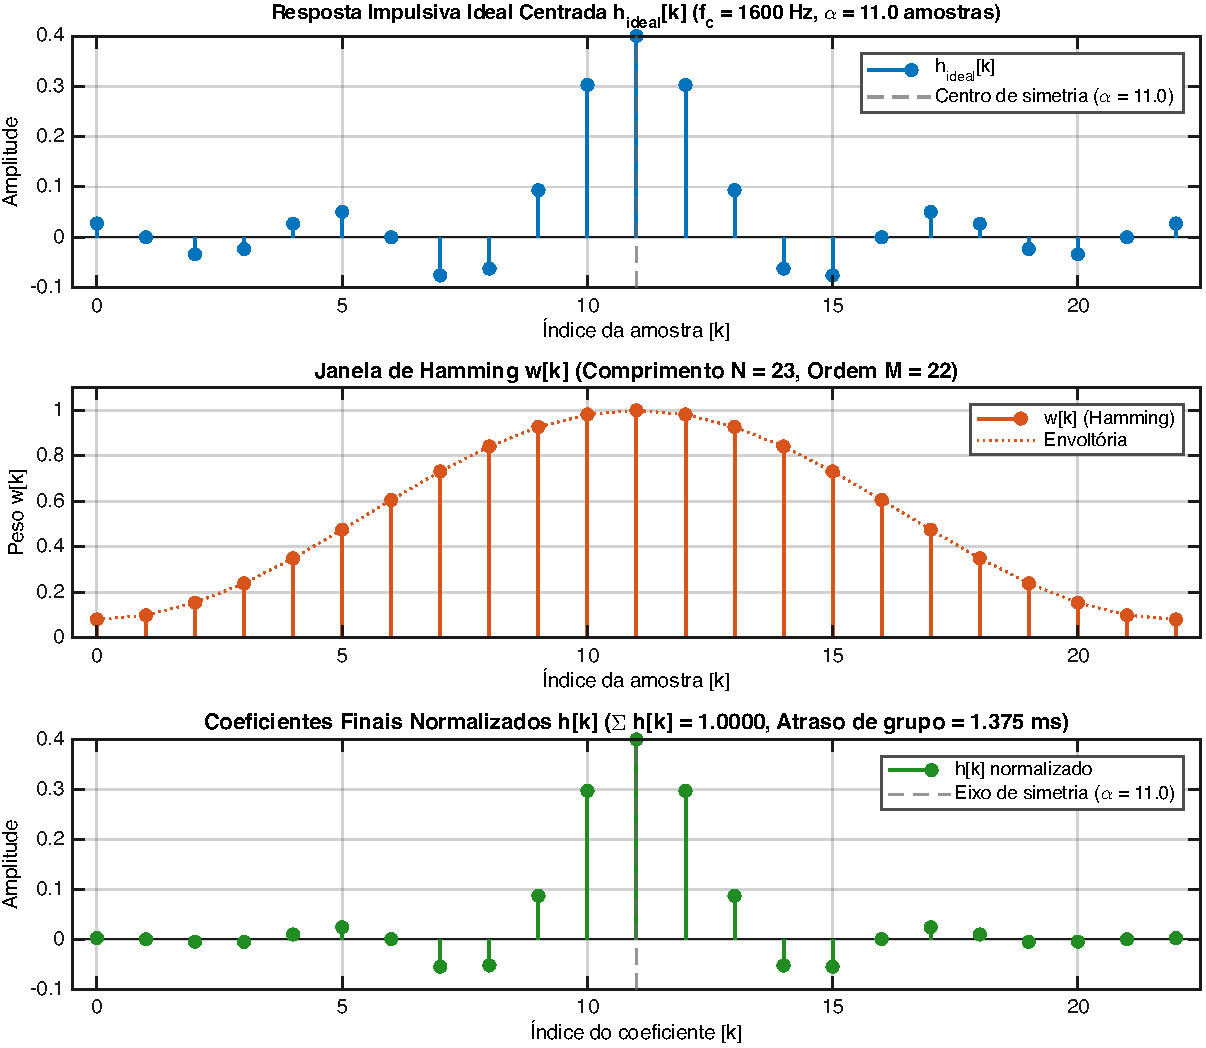
\includegraphics[width=0.88\linewidth, height=0.46\textheight, keepaspectratio]{fig_A1_impulso_janela.pdf}
    \caption{Etapa A: Resposta ideal truncada $h_{\text{ideal}}[k]$ centrada em $\alpha = 11$, janela de Hamming $w[k]$ ($N = 23$) e coeficientes normalizados $h[k]$.}
    \label{fig:A1_impulso}
\end{figure}

\begin{figure}[!htbp]
    \centering
    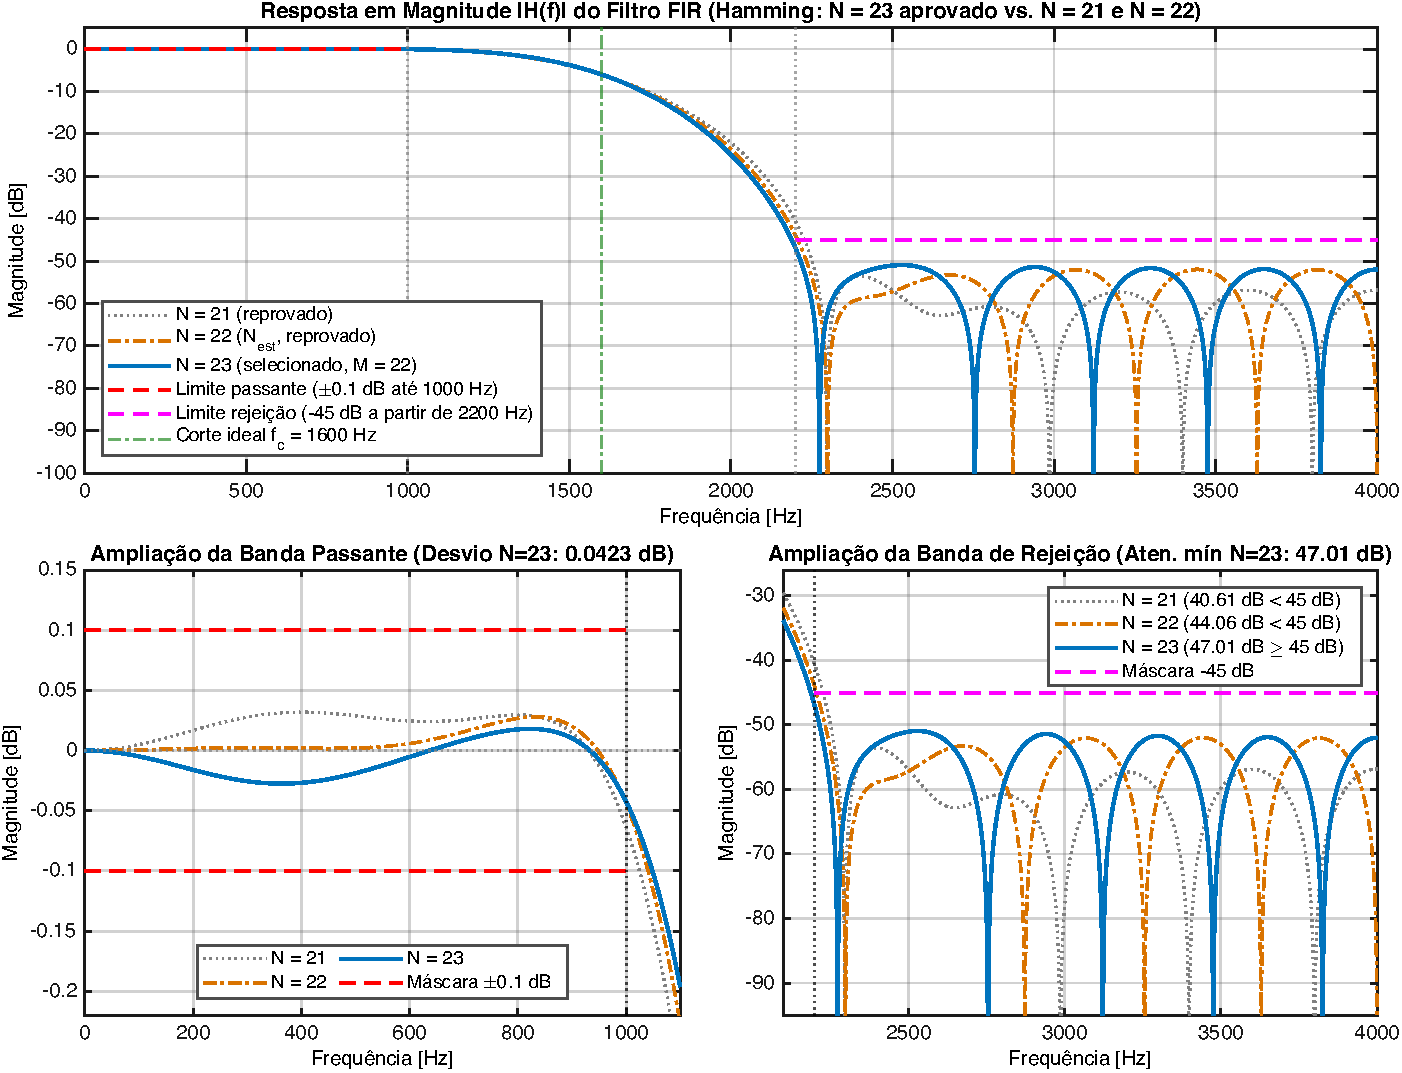
\includegraphics[width=0.92\linewidth, height=0.52\textheight, keepaspectratio]{fig_A2_magnitude_mascara.pdf}
    \caption{Etapa A: Magnitude $|H(f)|_{\text{dB}}$ para $N = 23$ comparada aos candidatos fronteiriços reprovados ($N = 21$ e $N = 22$), com ampliações nas bandas.}
    \label{fig:A2_magnitude}
\end{figure}

\subsection{Análise Técnica: Janelamento, Máscara, Normalização e Fase Linear}

\begin{itemize}[leftmargin=1.4em, itemsep=3pt]
    \item \textbf{Fenômeno de Gibbs e janela de Hamming:} Truncar a $\text{sinc}$ ideal com janela retangular convolui a resposta desejada com o núcleo de Dirichlet, cujo primeiro lóbulo lateral está apenas $\SI{13,5}{dB}$ ($\approx 3\pi/2$) abaixo do central, gerando oscilações de Gibbs ($\sim 9\%$) na borda de transição que persistem mesmo aumentando $M$~\cite{aula15, oppenheim2010}. Como o desempenho de uma janela depende da \textit{largura do lóbulo central} e do \textit{tamanho relativo dos lóbulos laterais}~\cite{aula15}, a janela de Hamming suaviza o truncamento e amplia a relação entre lóbulos para $\sim\SI{42}{dB}$ ($\sim\SI{53}{dB}$ no filtro integrado), ao compromisso inevitável de alargar a faixa de transição e exigir maior comprimento $N$~\cite{aula15, lyons2011}.

    \item \textbf{Estimativa de ordem vs.\ verificação da máscara:} A fórmula $N_{\text{est}} = 22$ aproxima somente a transição média da janela, sem impor simultaneamente os limites em $\SI{1000}{Hz}$ ($\pm\SI{0,10}{dB}$) e $\SI{2200}{Hz}$ ($\ge\SI{45,00}{dB}$). Conforme a Tabela~\ref{tab:A1_varredura} e a Figura~\ref{fig:A2_magnitude}, $N = 21$ e $N = 22$ cumprem a passante, porém \textbf{reprovam na borda $F_{\text{stop}} = \SI{2200}{Hz}$} ($\SI{40,6091}{dB}$ e $\SI{44,0615}{dB} < \SI{45,00}{dB}$), tornando indispensável a varredura em grade densa.

    \item \textbf{Justificativa de $N = 23$:} O acréscimo de um coeficiente ($N = 23$, $M = 22$) estreita o lóbulo principal para atingir $\SI{47,26}{dB}$ em $\SI{2200}{Hz}$ e mantém o primeiro lóbulo lateral ($\sim\SI{2612}{Hz}$) em $\SI{47,0065}{dB} \ge \SI{45,00}{dB}$, com $\delta_{p,\text{máx}} = \SI{0,042323}{dB}$. Como todo $N \le 22$ falha e $N \ge 24$ eleva latência e custo sem necessidade, $N = 23$ é o menor comprimento ótimo por janelamento.

    \item \textbf{Normalização DC (\texttt{h = h / sum(h)}):} Em $\omega = 0$, $H(e^{j0}) = \sum_{k=0}^{N-1} h[k]$~\cite{aula17}. Dividir pela soma corrige o truncamento ponderado e garante três efeitos~\cite{aula17}: ganho unitário ($\SI{0,000000}{dB}$) em DC, referência alinhada à máscara e preservação da forma relativa da resposta (zeros, simetria e fase inalterados) --- ressalvando-se que normalizar o DC não garante, por si só, que toda a passante cumpra $\pm\SI{0,10}{dB}$~\cite{aula17}.

    \item \textbf{Classificação Tipo I e fase linear por trechos:} Com simetria par ($h[k] = h[N-1-k]$), $K = 23$ ímpar e $M = 22$ par, o filtro é \textbf{Tipo I}~\cite{aula13, aula14} (distinto do Tipo~II de $K$ par, cujo atraso semi-inteiro ainda usa apenas atrasadores unitários $z^{-1}$~\cite{aula14}, e dos Tipos~III/IV antissimétricos). Isolando $h[11]$ e agrupando os pares simétricos:
    \begin{equation}
        H(e^{j\omega}) = A(\omega)\,e^{-j\omega M/2}, \qquad A(\omega) = h[11] + 2 \sum_{k=0}^{10} h[k] \cos\!\big(\omega (11 - k)\big) \in \mathbb{R}.
        \label{eq:fatoracao_tipo1}
    \end{equation}
    Pela Equação~\eqref{eq:fatoracao_tipo1}, a fase é \textbf{linear por trechos} ($\phi(\omega) = -11\omega$ para $A(\omega) > 0$, com saltos de $\pi$ nos zeros de $A(\omega)$ na rejeição)~\cite{aula14}, garantindo atraso de grupo constante $\tau_g = -\mathrm{d}\phi/\mathrm{d}\omega = M/2 = \SI{11,0}{amostras}$ ($\SI{1,3750}{ms}$) e ausência de distorção de fase na banda passante.
\end{itemize}

% ==============================================================================
% 4. ETAPA A2 — FILTER DESIGNER COMO FERRAMENTA AUXILIAR
% ==============================================================================
\FloatBarrier
\section{Etapa A2 — \textit{Filter Designer}: Janelamento vs.\ \textit{Equiripple}}

A inspeção de $h[k]$ ($N=23$) no \textit{Filter Designer} ($F_s = \SI{8000}{Hz}$) confirmou magnitude, fase linear, atraso de grupo plano ($\SI{11,0}{amostras}$) e $22$ zeros (pares recíprocos na passante e zeros sobre $|z|=1$ na rejeição). Projetou-se então na ferramenta um filtro \textbf{Equiripple} de ordem mínima para a mesma máscara via \textbf{algoritmo de Parks-McClellan} (troca de Remez / aproximação minimax de Chebyshev em \texttt{firpm}, salvo em \texttt{data/coeficientes\_equiripple.mat})~\cite{aula15, mathworks2026}, mantendo-se $h[k]$ ($N=23$) nas etapas B a E. A Tabela~\ref{tab:A2_equiripple} e a Figura~\ref{fig:A2_comp_eq} confrontam os resultados.

\begin{table}[!htbp]
    \centering
    \caption{Comparação de desempenho e custo computacional entre Janelamento (Hamming) e \textit{Equiripple} (\textit{Filter Designer}).}
    \label{tab:A2_equiripple}
    \small
    \renewcommand{\arraystretch}{1.08}
    \begin{adjustbox}{max width=\textwidth}
    \begin{tabular}{@{}lcc@{}}
        \toprule
        \textbf{Resultado / Métrica Comparativa} & \textbf{Janelamento (Hamming)} & \textbf{Equiripple (Parks-McClellan)} \\
        \midrule
        \textbf{Número de coeficientes ($N = K$)} & $\mathbf{\MetricaAN}$ & $\mathbf{\MetricaAIIEqN}$ \\
        Ordem do filtro ($M = N - 1$) & $\MetricaAOrdem$ & $\MetricaAIIEqOrdem$ \\
        \textbf{Desvio máximo na passante [\si{dB}]} ($\le \SI{0,10}{dB}$) & $\mathbf{\MetricaADesvioPassdB}$ & $\mathbf{\MetricaAIIEqDesvioPassdB}$ \\
        \textbf{Atenuação mínima na rejeição [\si{dB}]} ($\ge \SI{45,00}{dB}$) & $\mathbf{\MetricaAAtenStopdB}$ & $\mathbf{\MetricaAIIEqAtenStopdB}$ \\
        \textbf{Atende à máscara?} / Ganho DC [\si{dB}] & \textbf{Sim} / $\MetricaAGanhoDCdB\text{ dB}$ & \textbf{Sim} / $\MetricaAIIEqGanhoDCdB\text{ dB}$ ($\sum h = \MetricaAIIEqSomaCoefs$) \\
        Atraso de grupo constante ($\tau_g$) & $\MetricaAAtrasoAmostras\text{ amostras}$ ($\SI{1,3750}{ms}$) & $\MetricaAIIEqAtrasoAmostras\text{ amostras}$ ($\SI{0,8750}{ms}$, $-36,36\%$) \\
        Operações por amostra (MACs/amostra) & $23\text{ mult.} + 22\text{ somas}$ & $15\text{ mult.} + 14\text{ somas}$ \\
        Taxa de processamento em tempo real ($F_s = \SI{8}{kHz}$) & $\SI{184000}{MACs/s}$ & $\SI{120000}{MACs/s}$ ($\mathbf{-\MetricaAIIReducaoCoefsPerc\%}$) \\
        \bottomrule
    \end{tabular}
    \end{adjustbox}
\end{table}

\begin{figure}[!htbp]
    \centering
    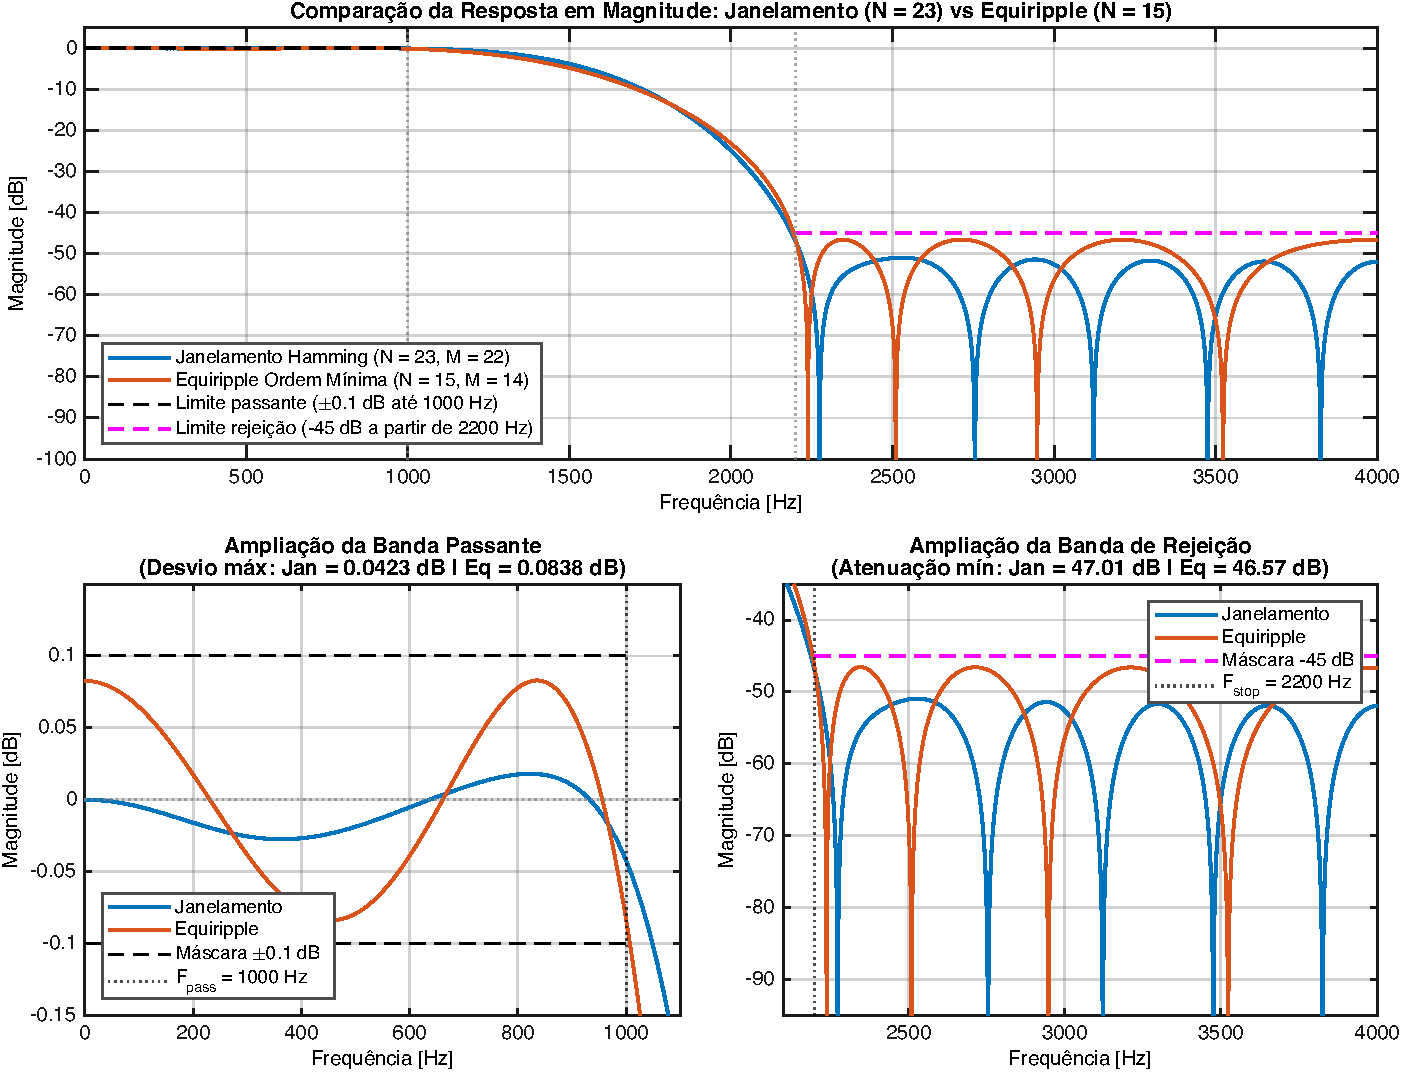
\includegraphics[width=0.92\linewidth, height=0.50\textheight, keepaspectratio]{fig_A2_comp_janelamento_equiripple.pdf}
    \caption{Etapa A2: Respostas em magnitude do filtro por Janelamento ($N = 23$) e do filtro \textit{Equiripple} de ordem mínima ($N = 15$), com ampliações nas bandas.}
    \label{fig:A2_comp_eq}
\end{figure}

\begin{enumerate}[leftmargin=1.4em, itemsep=3pt]
    \item \textbf{Distribuição espectral do erro:} O janelamento concentra o erro perto da transição e superdimensiona o interior das bandas (passante quase plana até $\SI{600}{Hz}$ e rejeição além de $\SI{-60}{dB}$ junto a $\SI{4000}{Hz}$). Pelo Teorema da Alternância de Chebyshev, o projeto \textit{Equiripple} distribui o erro uniformemente~\cite{aula15, manolakis2011}: todas as cristas na passante atingem $\pm\SI{0,083846}{dB}$ e todos os lóbulos na rejeição alinham-se em $\SI{-46,5690}{dB}$.
    \item \textbf{Impacto no custo computacional e latência:} Aproveitar integralmente as margens da máscara reduz o comprimento de $N = 23$ para $N_{\text{eq}} = 15$, economizando $\mathbf{\MetricaAIIReducaoCoefsPerc\%}$ dos MACs/s ($\SI{120000}{MACs/s}$ vs.\ $\SI{184000}{MACs/s}$), $8$ posições de memória e $4\text{ amostras}$ ($\SI{0,50}{ms}$) de atraso de grupo.
\end{enumerate}

% ==============================================================================
% 5. ETAPA B — IMPLEMENTAÇÃO COM BUFFER CIRCULAR
% ==============================================================================
\FloatBarrier
\section{Etapa B — Implementação com Buffer Circular (\texttt{fir\_circular})}

\subsection{Modos Operacionais e Arquitetura de Ponteiros}

A filtragem FIR realiza-se em modo \textbf{amostra por amostra} --- calculando cada saída $y[n]$ dentro de $T_s = 1/F_s = \SI{125}{\mu s}$ sem latência extra --- ou \textbf{bloco por bloco}, processando lotes de $B$ amostras (exigindo retenção de $M$ amostras nas fronteiras entre blocos e adicionando espera de $B-1$ amostras)~\cite{aula16}. A função \texttt{fir\_circular(x, h)} (\texttt{src/fir\_circular.m}) implementa o modo amostra por amostra sem chamar \texttt{filter}, \texttt{conv} ou \texttt{fftfilt} (Listagem~\ref{lst:fir_circular} e Figura~\ref{fig:tikz_buffer}).

\begin{lstlisting}[style=matlabstyle, float=!htbp, caption={Trecho essencial de \texttt{src/fir\_circular.m}: atualização anti-horária de \texttt{idx\_recente} e leitura horária com \texttt{idx\_leitura}.}, label={lst:fir_circular}]
buf = zeros(1, N);             % Buffer circular de N = 23 posicoes em repouso [amplitude]
y_lin = zeros(1, num_amostras);% Pre-alocacao do vetor de saida [amplitude]
idx_recente = 1;               % Ponteiro para a amostra mais recente (1..N) [indice]

for n = 1:num_amostras
    % 1. Escrita: avanca 1 posicao no sentido anti-horario (sobrescreve a mais antiga)
    idx_recente = idx_recente - 1;
    if idx_recente < 1, idx_recente = N; end
    buf(idx_recente) = x_lin(n);

    % 2. Leitura MAC: percorre no sentido horario a partir de idx_recente
    idx_leitura = idx_recente;
    acumulador  = 0.0;
    for k = 1:N
        acumulador = acumulador + h_lin(k) * buf(idx_leitura);
        idx_leitura = idx_leitura + 1;
        if idx_leitura > N, idx_leitura = 1; end
    end
    y_lin(n) = acumulador;     % Amostra filtrada y[n] [amplitude]
end
\end{lstlisting}

\begin{figure}[!htbp]
    \centering
    \begin{adjustbox}{width=0.86\textwidth}
    \begin{tikzpicture}[>=stealth, font=\small]
        \draw[thick, fill=gray!5] (0,0) circle (3.90cm);
        \draw[thick, fill=white]  (0,0) circle (2.20cm);
        \foreach \ang in {22.5, 67.5, 112.5, 157.5, 202.5, 247.5, 292.5, 337.5} {
            \draw[thick, gray!70] (\ang:2.20cm) -- (\ang:3.90cm);
        }
        \fill[blue!14] (67.5:2.20cm) arc (67.5:112.5:2.20cm) -- (112.5:3.90cm) arc (112.5:67.5:3.90cm) -- cycle;
        \draw[thick, blue!70!black] (67.5:2.20cm) arc (67.5:112.5:2.20cm) -- (112.5:3.90cm) arc (112.5:67.5:3.90cm) -- cycle;
        \fill[red!10] (112.5:2.20cm) arc (112.5:157.5:2.20cm) -- (157.5:3.90cm) arc (157.5:112.5:3.90cm) -- cycle;
        \draw[thick, red!60!black] (112.5:2.20cm) arc (112.5:157.5:2.20cm) -- (157.5:3.90cm) arc (157.5:112.5:3.90cm) -- cycle;

        \node[anchor=south,      font=\footnotesize\bfseries, text=blue!80!black] at (90:4.02cm)   {Pos.\ $1$};
        \node[anchor=south west, font=\footnotesize\bfseries, text=gray!80!black] at (45:4.00cm)   {Pos.\ $2$};
        \node[anchor=west,       font=\footnotesize\bfseries, text=gray!80!black] at (0:4.02cm)    {Pos.\ $3$};
        \node[anchor=north west, font=\footnotesize\bfseries, text=gray!80!black] at (-45:4.00cm)  {Pos.\ $4$};
        \node[anchor=north,      font=\footnotesize\bfseries, text=gray!80!black] at (-90:4.02cm)  {Pos.\ $5$};
        \node[anchor=north east, font=\footnotesize\bfseries, text=gray!80!black] at (-135:4.00cm) {$\cdots$};
        \node[anchor=east,       font=\footnotesize\bfseries, text=gray!80!black] at (180:4.02cm)  {Pos.\ $N\!-\!1$};
        \node[anchor=south east, font=\footnotesize\bfseries, text=red!75!black]  at (135:4.00cm)  {Pos.\ $N$};

        \node[align=center, font=\footnotesize] at (90:3.05cm)   {$\mathbf{x[n]}$\\[-1pt]{\scriptsize $\times\, h[1]$}};
        \node[align=center, font=\footnotesize] at (45:3.05cm)   {$x[n-1]$\\[-1pt]{\scriptsize $\times\, h[2]$}};
        \node[align=center, font=\footnotesize] at (0:3.05cm)    {$x[n-2]$\\[-1pt]{\scriptsize $\times\, h[3]$}};
        \node[align=center, font=\footnotesize] at (-45:3.05cm)  {$x[n-3]$\\[-1pt]{\scriptsize $\times\, h[4]$}};
        \node[align=center, font=\footnotesize] at (-90:3.05cm)  {$x[n-4]$\\[-1pt]{\scriptsize $\times\, h[5]$}};
        \node[align=center, font=\footnotesize] at (-135:3.05cm) {$\cdots$};
        \node[align=center, font=\scriptsize]   at (180:3.05cm)  {$x[n\!-\!N\!+\!2]$\\[-1pt]{$\times\, h[N\!-\!1]$}};
        \node[align=center, font=\scriptsize]   at (135:3.05cm)  {$x[n\!-\!N\!+\!1]$\\[-1pt]{$\times\, h[N]$}};

        \draw[->, ultra thick, blue!80!black] (90:5.35cm) -- (90:4.56cm);
        \node[above, align=center, font=\footnotesize\bfseries, text=blue!80!black] at (90:5.35cm)
            {\texttt{idx\_recente} ($x[n]$)};

        \draw[->, very thick, red!75!black, dashed] (106:4.85cm) arc (106:128:4.85cm);
        \node[draw=red!60!black, fill=red!5, rounded corners=3pt, inner sep=5pt,
              text width=4.4cm, align=flush left, font=\scriptsize, anchor=south east] at (-3.65, 3.85)
            {\textbf{\textcolor{red!75!black}{Escrita (anti-horário)}}\\
             \texttt{idx\_recente = idx\_recente - 1}\\
             Sobrescreve $x[n-N+1]$ na Pos.\ $N$.};

        \draw[->, very thick, green!50!black] (74:4.95cm) arc (74:16:4.95cm);
        \node[draw=green!50!black, fill=green!5, rounded corners=3pt, inner sep=5pt,
              text width=4.5cm, align=flush left, font=\scriptsize, anchor=south west] at (3.65, 3.85)
            {\textbf{\textcolor{green!45!black}{Leitura MAC (sentido horário)}}\\
             \texttt{idx\_leitura = idx\_leitura + 1}\\
             Percorre $k = 1 \dots N$ sem mover dados.};

        \node[align=center, font=\scriptsize] at (0,0)
            {\textbf{\footnotesize Buffer Circular}\\
             \textbf{($N = 23$ posições)}\\[2pt]
             Numeração horária $1 \rightarrow N$\\[2pt]
             $y[n] = \sum_{k=1}^{N} h[k]\,\text{buf}(i_L)$};

        \node[draw=gray!60, fill=gray!12, minimum width=1.65cm, minimum height=0.52cm, font=\scriptsize\bfseries] at (-6.85, -5.55) {Posição};
        \node[draw=gray!60, fill=gray!12, minimum width=1.65cm, minimum height=0.56cm, font=\scriptsize\bfseries] at (-6.85, -6.11) {Conteúdo};
        \node[draw=gray!60, fill=gray!12, minimum width=1.65cm, minimum height=0.52cm, font=\scriptsize\bfseries] at (-6.85, -6.67) {Peso MAC};

        \begin{scope}[
            celpos/.style={draw=gray!60, minimum width=1.70cm, minimum height=0.52cm, font=\scriptsize\bfseries},
            celsamp/.style={draw=gray!60, minimum width=1.70cm, minimum height=0.56cm, font=\scriptsize},
            celcoef/.style={draw=gray!60, minimum width=1.70cm, minimum height=0.52cm, font=\scriptsize}
        ]
            \node[celpos,  fill=blue!14, text=blue!80!black] at (-5.15, -5.55) {Pos.\ $1$};
            \node[celsamp, fill=blue!14]                     at (-5.15, -6.11) {$\mathbf{x[n]}$};
            \node[celcoef, fill=blue!14]                     at (-5.15, -6.67) {$\times\, h[1]$};
            \node[celpos,  fill=gray!5]  at (-3.45, -5.55) {Pos.\ $2$};
            \node[celsamp, fill=gray!5]  at (-3.45, -6.11) {$x[n-1]$};
            \node[celcoef, fill=gray!5]  at (-3.45, -6.67) {$\times\, h[2]$};
            \node[celpos,  fill=gray!5]  at (-1.75, -5.55) {Pos.\ $3$};
            \node[celsamp, fill=gray!5]  at (-1.75, -6.11) {$x[n-2]$};
            \node[celcoef, fill=gray!5]  at (-1.75, -6.67) {$\times\, h[3]$};
            \node[celpos,  fill=gray!5]  at (-0.05, -5.55) {Pos.\ $4$};
            \node[celsamp, fill=gray!5]  at (-0.05, -6.11) {$x[n-3]$};
            \node[celcoef, fill=gray!5]  at (-0.05, -6.67) {$\times\, h[4]$};
            \node[celpos,  fill=gray!5]  at (1.65, -5.55)  {Pos.\ $5$};
            \node[celsamp, fill=gray!5]  at (1.65, -6.11)  {$x[n-4]$};
            \node[celcoef, fill=gray!5]  at (1.65, -6.67)  {$\times\, h[5]$};
            \node[celpos,  fill=gray!5]  at (3.35, -5.55)  {$\cdots$};
            \node[celsamp, fill=gray!5]  at (3.35, -6.11)  {$\cdots$};
            \node[celcoef, fill=gray!5]  at (3.35, -6.67)  {$\cdots$};
            \node[celpos,  fill=gray!5]  at (5.05, -5.55)  {Pos.\ $N\!-\!1$};
            \node[celsamp, fill=gray!5]  at (5.05, -6.11)  {$x[n\!-\!N\!+\!2]$};
            \node[celcoef, fill=gray!5]  at (5.05, -6.67)  {$\times\, h[N\!-\!1]$};
            \node[celpos,  fill=red!10, text=red!75!black] at (6.75, -5.55) {Pos.\ $N$};
            \node[celsamp, fill=red!10]                    at (6.75, -6.11) {$x[n\!-\!N\!+\!1]$};
            \node[celcoef, fill=red!10]                    at (6.75, -6.67) {$\times\, h[N]$};
        \end{scope}
        \draw[->, thick, red!75!black, dashed] (-5.15, -5.29) -- (-5.15, -4.92) -- (6.75, -4.92) -- (6.75, -5.29);
        \node[fill=white, inner sep=2pt, font=\scriptsize\bfseries, text=red!75!black] at (0.80, -4.92)
            {Próxima escrita (\texttt{idx\_recente}): $1 \rightarrow N$ (\textit{wrap-around})};
        \draw[->, thick, green!50!black] (-5.15, -7.12) -- (6.75, -7.12);
        \node[below, font=\scriptsize\bfseries, text=green!45!black] at (0.80, -7.12)
            {Percurso de leitura ($i_L \equiv \text{\texttt{idx\_leitura}}$): $1 \rightarrow 2 \rightarrow \cdots \rightarrow N$};
    \end{tikzpicture}
    \end{adjustbox}
    \caption{Etapa B: Esquema do buffer circular ($N = 23$) numerado no sentido horário e seu mapeamento linear equivalente no instante $n$.}
    \label{fig:tikz_buffer}
\end{figure}

\subsection{Validação Temporal, Espectral e Análise Técnica}

Validou-se \texttt{fir\_circular(x, h)} frente a \texttt{filter(h, 1, x)} em dois testes (Tabela~\ref{tab:B1_validacao}): (1) \textbf{impulso unitário} ($L=43$), recuperando exatamente $h[k]$ em $n = 0 \dots 22$ e repouso nulo em $n \ge 23$ (Figura~\ref{fig:B1_impulso}); e (2) \textbf{duas senoides} ($\SI{500}{Hz} + \SI{3000}{Hz}$, $L=400$), onde após o transitório de $M = 22\text{ amostras}$ ($\SI{2,75}{ms}$)~\cite{aula16} o tom de $\SI{3000}{Hz}$ cai em $\SI{-52,58}{dB}$ e o de $\SI{500}{Hz}$ emerge atrasado de $\tau_g = \SI{11,0}{amostras}$ ($\SI{1,375}{ms}$), diferindo de \texttt{filter} apenas em $\MetricaBErroMaxSenFilter$ (Figura~\ref{fig:B2_senoides}).

\begin{table}[!htbp]
    \centering
    \caption{Validação temporal de \texttt{fir\_circular} vs.\ \texttt{filter} e ganhos espectrais pontuais via \texttt{freqz}.}
    \label{tab:B1_validacao}
    \small
    \setlength{\tabcolsep}{5pt}
    \renewcommand{\arraystretch}{1.08}
    \begin{adjustbox}{max width=\textwidth}
    \begin{tabular}{@{}lccc@{}}
        \toprule
        \textbf{Cenário / Frequência Avaliada} & \textbf{Janela / Ganho $|H(f)|$} & \textbf{Erro Máx.\ / Ganho [\si{dB}]} & \textbf{Veredito} \\
        \midrule
        Impulso $\delta[n]$ ($y_{\text{circ}}$ vs.\ \texttt{filter} e vs.\ $h[k]$) & $43\text{ amostras}$ & $\num{0,000000e+00}$ & Equivalência exata \\
        Cauda nula pós-impulso ($n = 23 \dots 42$) & $20\text{ amostras}$ & $\num{0,000000e+00}$ & Repouso exato \\
        Duas senoides ($\SI{500}{Hz} + \SI{3000}{Hz}$ vs.\ \texttt{filter}) & $400\text{ amostras}$ ($\SI{50}{ms}$) & $\num{3,330669e-16}$ & Precisão \texttt{double} \\
        \midrule
        $f_1 = \SI{500}{Hz}$ (Banda Passante via \texttt{freqz}) & $\MetricaBGanhoPassLin$ & $\MetricaBGanhoPassdB\text{ dB}$ ($|\Delta| \le \SI{0,10}{dB}$) & \textbf{Atende} \\
        $f_2 = \SI{3000}{Hz}$ (Banda de Rejeição via \texttt{freqz}) & $\MetricaBGanhoStopLin$ & $\MetricaBGanhoStopdB\text{ dB}$ ($A_s \ge \SI{45,00}{dB}$) & \textbf{Atende} \\
        \bottomrule
    \end{tabular}
    \end{adjustbox}
\end{table}

\begin{figure}[!htbp]
    \centering
    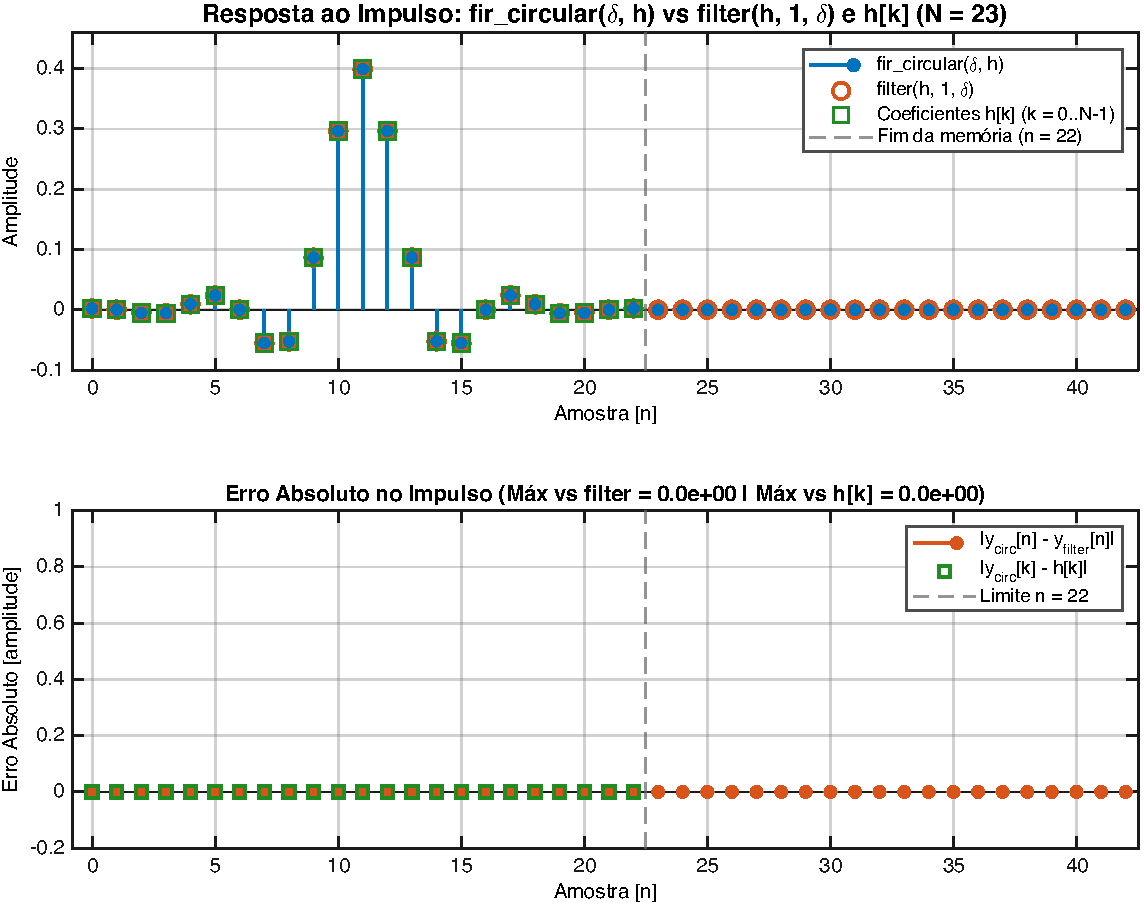
\includegraphics[width=0.88\linewidth, height=0.45\textheight, keepaspectratio]{fig_B1_impulso_comparacao.pdf}
    \caption{Etapa B: Resposta ao impulso unitário de \texttt{fir\_circular} comparada a $h[k]$ e \texttt{filter} ($L = 43$ amostras).}
    \label{fig:B1_impulso}
\end{figure}

\begin{figure}[!htbp]
    \centering
    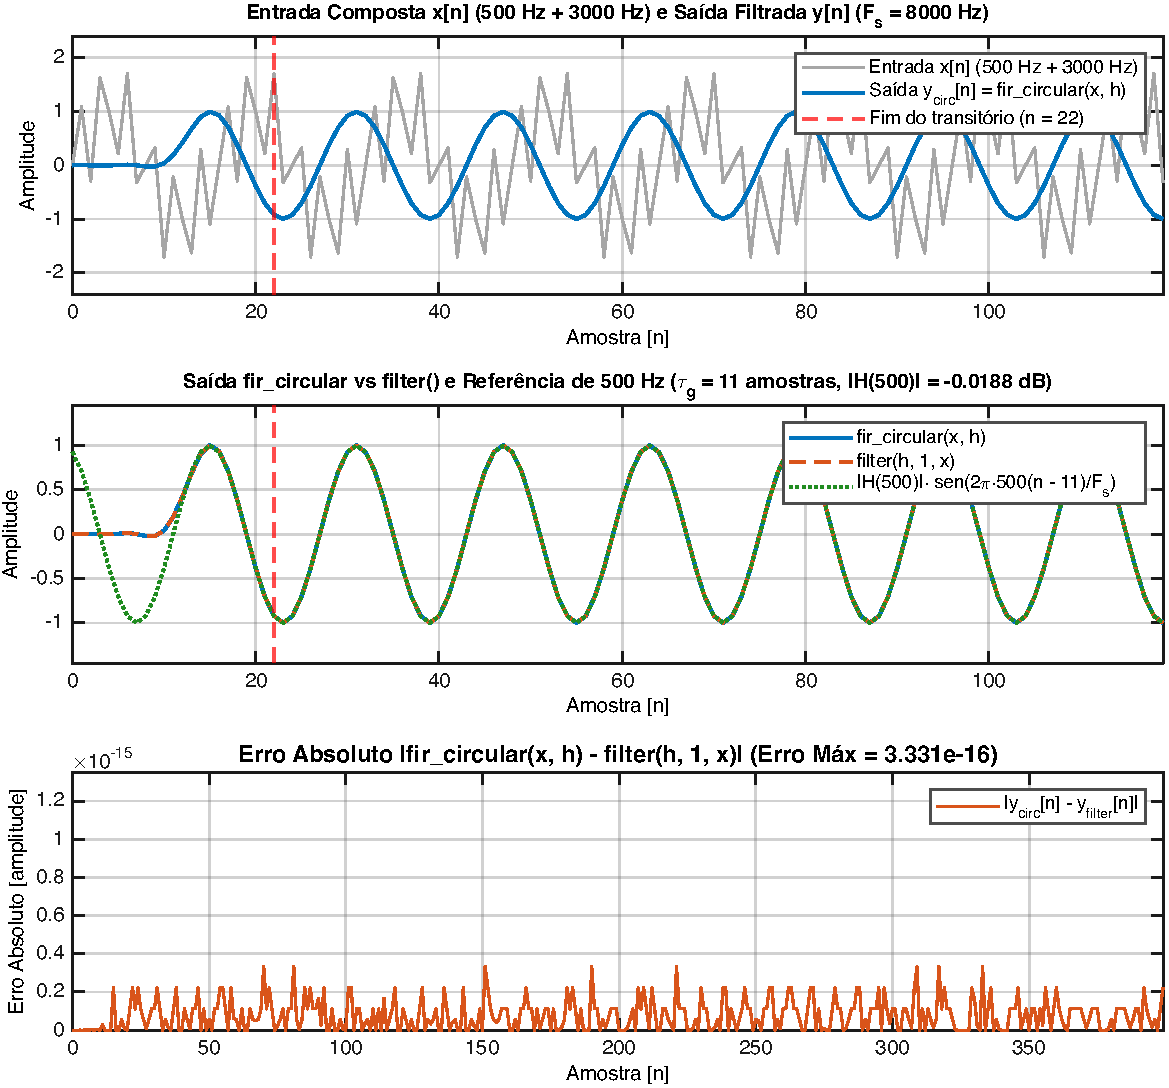
\includegraphics[width=0.92\linewidth, height=0.54\textheight, keepaspectratio]{fig_B2_senoides_temporal.pdf}
    \caption{Etapa B: Filtragem temporal de $\SI{500}{Hz} + \SI{3000}{Hz}$, destacando transitório ($22\text{ amostras}$), atraso $\tau_g = 11\text{ amostras}$ e resíduo $\sim 10^{-16}$.}
    \label{fig:B2_senoides}
\end{figure}

\begin{itemize}[leftmargin=1.4em, itemsep=3pt]
    \item \textbf{Eliminação de cópias de memória ($O(1)$ vs.\ $O(N)$):} Na linha de atraso linear, cada amostra exige $M = 22$ deslocamentos físicos ($\text{buf}[k]\leftarrow\text{buf}[k-1]$). No buffer circular, as amostras permanecem fixas e apenas \texttt{idx\_recente} é decrementado em $O(1)$ para sobrescrever $x[n-N]$~\cite{aula16, lyons2011} (em DSPs, um segundo buffer circular percorre $b_0 \dots b_M$ em hardware~\cite{aula16}).
    \item \textbf{Pareamento $h[k]\,x[n-k+1]$:} Como a escrita recua no sentido \textbf{anti-horário}, as amostras passadas ficam dispostas no sentido \textbf{horário} a partir de \texttt{idx\_recente}. Avançar \texttt{idx\_leitura} no sentido horário ($k = 1 \dots N$) associa exatamente $h[k]$ a $x[n-k+1]$.
    \item \textbf{Validação algorítmica vs.\ máscara:} Coincidir com \texttt{filter} prova apenas a correção da soma de convolução, pois \texttt{filter} processaria sem erro numérico mesmo um vetor reprovado ($N=22$), e dois tons isolados não testam as bordas críticas ($1000$ e $\SI{2200}{Hz}$).
    \item \textbf{Exploração da simetria Tipo I:} O buffer circular reduz a movimentação de memória, mas não diminui por si só o número de multiplicações ($K = 23$)~\cite{aula16}. Contudo, pré-somando pares simétricos $b_k(x[n-k]+x[n-M+k])$ com dois ponteiros percorrendo o anel em sentidos opostos até o centro, reduzem-se as multiplicações para $(K+1)/2 = 12$ ($-47,8\%$), mantendo $M = 22$ atrasos~\cite{aula14, aula16}.
\end{itemize}

% ==============================================================================
% 6. ETAPA C — QUANTIZAÇÃO DOS COEFICIENTES
% ==============================================================================
\FloatBarrier
\section{Etapa C — Quantização dos Coeficientes (\texttt{Q1.15} e \texttt{Q1.7})}

Na notação em complemento de dois \texttt{Qn.m} (par \texttt{[B m]} no MATLAB, ex.\ \texttt{[16 15]} para $15$ bits fracionários, com passo $\Delta = 2^{-m}$), separam-se \textbf{erros de quantização} (coeficientes/amostras) e \textbf{erros aritméticos}~\cite{aula17}. Isolando a quantização dos coeficientes, arredondou-se $h[k]$ (\texttt{double}) em múltiplos inteiros de $\Delta$ sem renormalização para \texttt{Q1.15} ($F=15$, $\Delta_{15} = 2^{-15} \approx \num{3,0518e-5}$) e \texttt{Q1.7} ($F=7$, $\Delta_7 = 2^{-7} = 1/128 = \num{0,0078125}$; ex.\ $h[5] = 0,02390682 \approx 3,06\Delta_7 \to 3/128 = 0,02343750$, erro $-4,693\times 10^{-4}$~\cite{aula17}):
\begin{equation}
    h_Q[k] = \frac{\text{round}\!\left(h[k] \cdot 2^F\right)}{2^F}, \quad e_Q[k] = h_Q[k] - h[k] \;\Longrightarrow\; H_Q(e^{j\omega}) = H(e^{j\omega}) + E(e^{j\omega}).
    \label{eq:hq_decomp}
\end{equation}
Diferentemente de filtros IIR --- onde perturbações podem deslocar polos próximos da circunferência de raio unitário (CRU) para o exterior e tornar o filtro instável ---, filtros FIR preservam incondicionalmente a estabilidade BIBO~\cite{aula17}. As Tabelas~\ref{tab:C1_coeficientes} e~\ref{tab:C2_metricas} e a Figura~\ref{fig:C1_quant_coef} reúnem os resultados.

\begin{table}[!htbp]
    \centering
    \caption{Coeficientes originais $h[k]$ ($N = 23$) e versões quantizadas em \texttt{Q1.7} e \texttt{Q1.15} com erros individuais $e_Q[k] = h_Q[k] - h[k]$.}
    \label{tab:C1_coeficientes}
    \scriptsize
    \setlength{\tabcolsep}{5pt}
    \renewcommand{\arraystretch}{1.04}
    \begin{adjustbox}{max width=\textwidth}
    \begin{tabular}{@{}crrrrr@{}}
        \toprule
        \textbf{Índice ($k$)} & \multicolumn{1}{c}{\textbf{$h[k]$ (\texttt{double})}} & \multicolumn{1}{c}{\textbf{$h_{\text{Q1.7}}[k]$}} & \multicolumn{1}{c}{\textbf{Erro $e_{\text{Q1.7}}[k]$}} & \multicolumn{1}{c}{\textbf{$h_{\text{Q1.15}}[k]$}} & \multicolumn{1}{c}{\textbf{Erro $e_{\text{Q1.15}}[k]$}} \\
        \midrule
        \rowcolor{rowfail}
        0  & $+0,00219838$ & $+0,00000000$ & $-2,198376\times 10^{-3}$ & $+0,00219727$ & $-1,110097\times 10^{-6}$ \\
        1  & $-1,5357\times 10^{-18}$ & $0,00000000$ & $+1,535651\times 10^{-18}$ & $0,00000000$ & $+1,535651\times 10^{-18}$ \\
        2  & $-0,00513949$ & $-0,00781250$ & $\mathbf{-2,673012\times 10^{-3}}$ & $-0,00512695$ & $+1,253520\times 10^{-5}$ \\
        3  & $-0,00557566$ & $-0,00781250$ & $-2,236844\times 10^{-3}$ & $-0,00558472$ & $-9,061077\times 10^{-6}$ \\
        4  & $+0,00931175$ & $+0,00781250$ & $-1,499248\times 10^{-3}$ & $+0,00930786$ & $-3,886926\times 10^{-6}$ \\
        5  & $+0,02390682$ & $+0,02343750$ & $-4,693181\times 10^{-4}$ & $+0,02389526$ & $-1,155439\times 10^{-5}$ \\
        6  & $-9,4267\times 10^{-18}$ & $0,00000000$ & $+9,426665\times 10^{-18}$ & $0,00000000$ & $+9,426665\times 10^{-18}$ \\
        7  & $-0,05524793$ & $-0,05468750$ & $+5,604296\times 10^{-4}$ & $-0,05523682$ & $+1,111321\times 10^{-5}$ \\
        8  & $-0,05238580$ & $-0,05468750$ & $-2,301705\times 10^{-3}$ & $-0,05239868$ & $-1,288655\times 10^{-5}$ \\
        9  & $+0,08658761$ & $+0,08593750$ & $-6,501124\times 10^{-4}$ & $+0,08657837$ & $-9,243257\times 10^{-6}$ \\
        10 & $+0,29664427$ & $+0,29687500$ & $+2,307295\times 10^{-4}$ & $+0,29663086$ & $-1,341114\times 10^{-5}$ \\
        \rowcolor{rowpass}
        11 & $+0,39940009$ & $+0,39843750$ & $-9,625876\times 10^{-4}$ & $+0,39941406$ & $\mathbf{+1,397490\times 10^{-5}}$ \\
        12 & $+0,29664427$ & $+0,29687500$ & $+2,307295\times 10^{-4}$ & $+0,29663086$ & $-1,341114\times 10^{-5}$ \\
        13 & $+0,08658761$ & $+0,08593750$ & $-6,501124\times 10^{-4}$ & $+0,08657837$ & $-9,243257\times 10^{-6}$ \\
        14 & $-0,05238580$ & $-0,05468750$ & $-2,301705\times 10^{-3}$ & $-0,05239868$ & $-1,288655\times 10^{-5}$ \\
        15 & $-0,05524793$ & $-0,05468750$ & $+5,604296\times 10^{-4}$ & $-0,05523682$ & $+1,111321\times 10^{-5}$ \\
        16 & $-9,4267\times 10^{-18}$ & $0,00000000$ & $+9,426665\times 10^{-18}$ & $0,00000000$ & $+9,426665\times 10^{-18}$ \\
        17 & $+0,02390682$ & $+0,02343750$ & $-4,693181\times 10^{-4}$ & $+0,02389526$ & $-1,155439\times 10^{-5}$ \\
        18 & $+0,00931175$ & $+0,00781250$ & $-1,499248\times 10^{-3}$ & $+0,00930786$ & $-3,886926\times 10^{-6}$ \\
        19 & $-0,00557566$ & $-0,00781250$ & $-2,236844\times 10^{-3}$ & $-0,00558472$ & $-9,061077\times 10^{-6}$ \\
        20 & $-0,00513949$ & $-0,00781250$ & $\mathbf{-2,673012\times 10^{-3}}$ & $-0,00512695$ & $+1,253520\times 10^{-5}$ \\
        21 & $-1,5357\times 10^{-18}$ & $0,00000000$ & $+1,535651\times 10^{-18}$ & $0,00000000$ & $+1,535651\times 10^{-18}$ \\
        \rowcolor{rowfail}
        22 & $+0,00219838$ & $+0,00000000$ & $-2,198376\times 10^{-3}$ & $+0,00219727$ & $-1,110097\times 10^{-6}$ \\
        \bottomrule
    \end{tabular}
    \end{adjustbox}
\end{table}

\begin{table}[!htbp]
    \centering
    \caption{Métricas de erro de quantização de coeficientes e desempenho espectral para as três versões ($N = 23$).}
    \label{tab:C2_metricas}
    \small
    \setlength{\tabcolsep}{5pt}
    \renewcommand{\arraystretch}{1.07}
    \begin{adjustbox}{max width=\textwidth}
    \begin{tabular}{@{}lccc@{}}
        \toprule
        \textbf{Métrica Avaliada} & \textbf{Original (\texttt{double})} & \textbf{Quantizado \texttt{Q1.15}} & \textbf{Quantizado \texttt{Q1.7}} \\
        \midrule
        Passo ($\Delta = 2^{-F}$) / Limite ($\Delta / 2$) & $\num{2,22e-16}$ / $\num{1,11e-16}$ & $\num{3,0518e-5}$ / $\num{1,5259e-5}$ & $\num{7,8125e-3}$ / $\num{3,9063e-3}$ \\
        \textbf{Erro absoluto máximo ($\max_k |e_Q[k]|$)} & $\num{0,000000e+00}$ & $\mathbf{\MetricaCErroMaxQXV}$ & $\mathbf{\MetricaCErroMaxQVII}$ \\
        \textbf{Erro quadrático médio (EQM)} & $\num{0,000000e+00}$ & $\mathbf{\MetricaCEQMQXV}$ & $\mathbf{\MetricaCEQMQVII}$ \\
        Coeficientes iguais a zero & $0$ ($4 \approx 10^{-18}$) & $4$ ($k \in \{1,6,16,21\}$) & $6$ ($k \in \{0,1,6,16,21,22\}$) \\
        Erro máximo de simetria & $\num{0,0000e+00}$ & $\num{0,0000e+00}$ & $\num{0,0000e+00}$ \\
        \textbf{Soma dos coeficientes ($\sum_{k=0}^{22} h_Q[k]$)} & $1,00000000$ & $\MetricaCSomaQXV$ ($32766/32768$) & $\MetricaCSomaQVII$ ($125/128$) \\
        \textbf{Ganho DC ($20\log_{10}|\sum h_Q[k]|$) [\si{dB}]} & $\SI{0,000000}{dB}$ & $\mathbf{\MetricaCGanhoDCQXVdB\text{ \textbf{dB}}}$ & $\mathbf{\MetricaCGanhoDCQVIIdB\text{ \textbf{dB}}}$ \\
        \textbf{Desvio máximo na passante [\si{dB}]} ($\le 0,10$) & $\SI{0,042323}{dB}$ & $\mathbf{\MetricaCDesvioPassQXVdB\text{ \textbf{dB}}}$ & $\mathbf{\MetricaCDesvioPassQVIIdB\text{ \textbf{dB}}}$ (\textbf{Reprova}) \\
        \textbf{Atenuação mínima na rejeição [\si{dB}]} ($\ge 45,00$) & $\SI{47,0065}{dB}$ & $\mathbf{\MetricaCAtenStopQXVdB\text{ \textbf{dB}}}$ & $\mathbf{\MetricaCAtenStopQVIIdB\text{ \textbf{dB}}}$ (\textbf{Reprova}) \\
        \textbf{Atende à máscara?} & \textbf{Sim} & \textbf{Sim} & \textbf{Não} \\
        \bottomrule
    \end{tabular}
    \end{adjustbox}
\end{table}

\begin{figure}[!htbp]
    \centering
    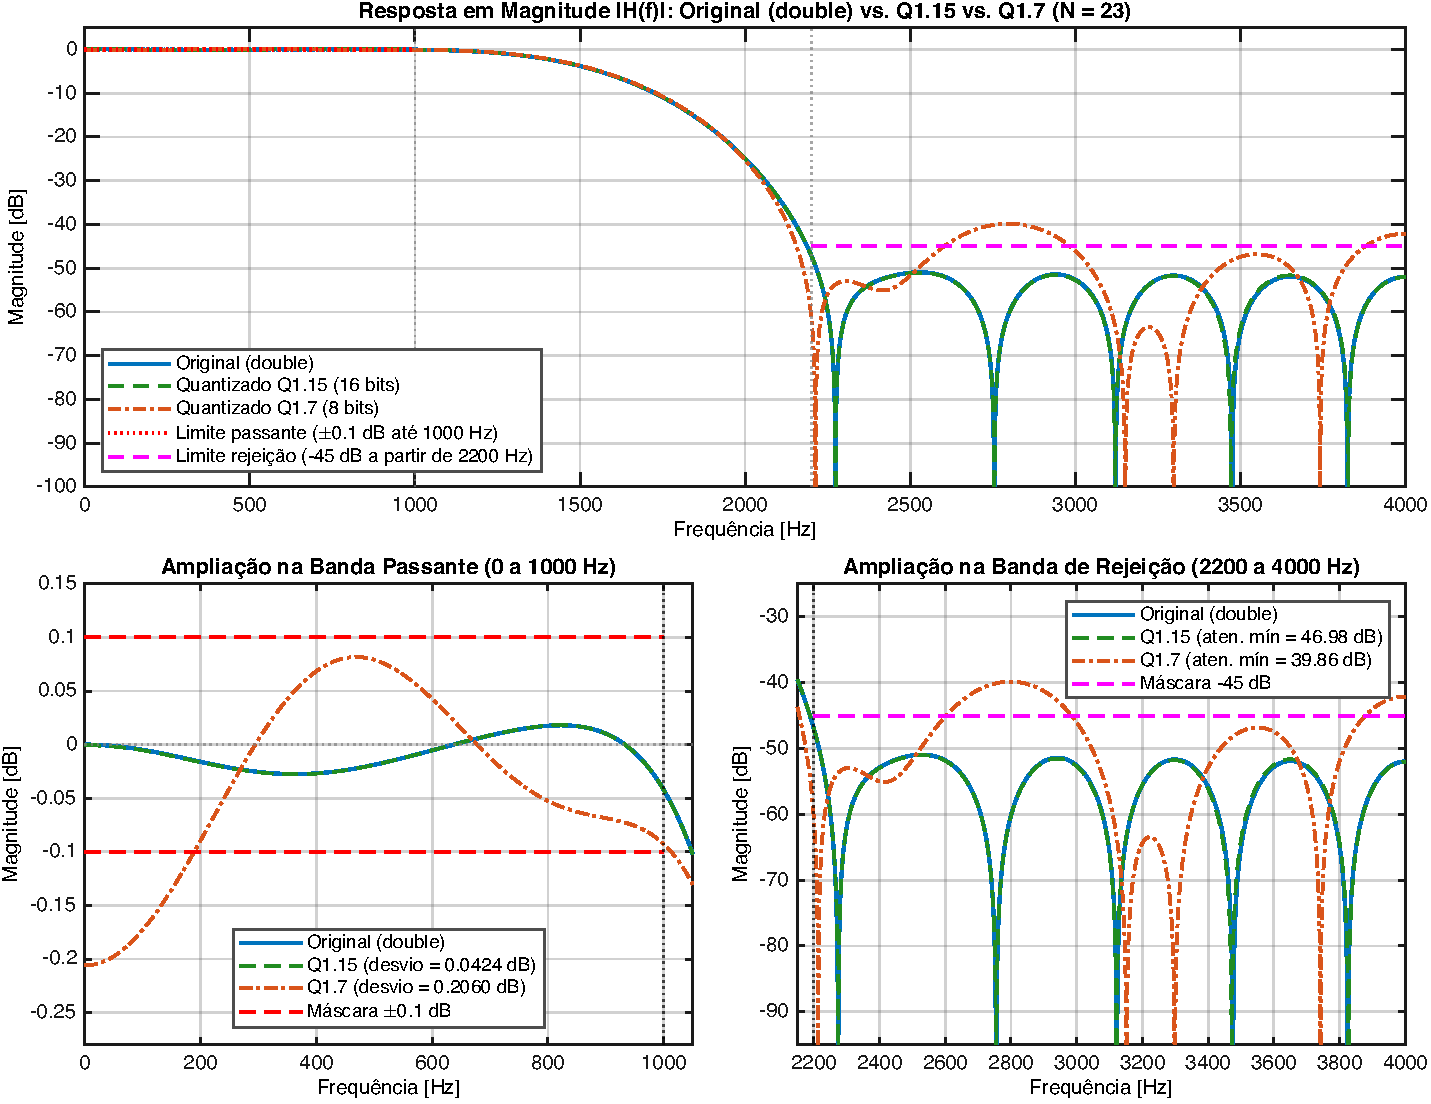
\includegraphics[width=0.92\linewidth, height=0.50\textheight, keepaspectratio]{fig_C1_respostas_quant_coef.pdf}
    \caption{Etapa C: Comparação das respostas em magnitude entre o filtro original (\texttt{double}), em \texttt{Q1.15} e em \texttt{Q1.7}, com ampliações nas bandas.}
    \label{fig:C1_quant_coef}
\end{figure}

\subsection{Respostas às Questões de Análise (Etapa C)}

\begin{enumerate}[leftmargin=1.5em, itemsep=3pt]
    \item \textbf{Coeficientes mais alterados:} Em erro absoluto, o máximo em \texttt{Q1.7} ocorreu no par $k = 2, 20$ ($\MetricaCErroMaxQVII$, $68,4\%$ de $\Delta_7/2$) e em \texttt{Q1.15} no termo central $k = 11$ ($\MetricaCErroMaxQXV$, $91,6\%$ de $\Delta_{15}/2$). Em erro relativo, as caudas sofreram os maiores desvios em \texttt{Q1.7} ($100\%$ em $k=0,22$ e $52,0\%$ em $k=2,20$) por possuírem amplitude comparável ao passo $\Delta_7$.
    \item \textbf{Coeficientes zerados:} Além dos $4$ zeros analíticos da $\text{sinc}$ ($k \in \{1,6,16,21\}$), em \texttt{Q1.7} a zona morta $|h[k]| < \Delta_7/2 = 0,00390625$ anulou também as extremidades não nulas $k = 0$ e $k = 22$ ($|h[0]| = 0,00219838$), reduzindo o suporte ativo para $19$ amostras; em \texttt{Q1.15} ($\Delta_{15}/2 \approx \num{1,53e-5}$), as extremidades foram preservadas ($72/32768$).
    \item \textbf{Preservação da simetria:} \textbf{Sim} ($\max|h_Q[k]-h_Q[N-1-k]| = 0$), pois o operador determinístico $Q(\cdot)$ mapeia valores simétricos idênticos $h[k]=h[N-1-k]$ no mesmo nível quantizado~\cite{aula17}.
    \item \textbf{Consequência para a fase:} Mantida a simetria par, ambos permanecem FIR \textbf{Tipo I} com \textbf{fase estritamente linear por trechos} e $\tau_g = \SI{11,0}{amostras}$ ($\SI{1,3750}{ms}$), perturbando-se apenas $A_Q(\omega)$ e os zeros~\cite{aula17}.
    \item \textbf{Banda mais afetada:} A \textbf{banda de rejeição}, onde $|H(e^{j\omega})| \le 0,00446$ depende de cancelamento fino e $|E(e^{j\omega})|$ em \texttt{Q1.7} reduz a atenuação mínima em $\SI{7,14}{dB}$ (para $\SI{39,8632}{dB} < \SI{45}{dB}$); na passante, $\sum e_{\text{Q1.7}}[k] = -3/128$ desloca a curva em $\SI{-0,205999}{dB}$, violando $\pm\SI{0,10}{dB}$.
    \item \textbf{Atendimento à máscara:} Apenas \textbf{Original (\texttt{double})} e \textbf{\texttt{Q1.15}} ($\delta_{p,\text{máx}} = \SI{0,042440}{dB}$, $A_{s,\text{mín}} = \SI{46,9752}{dB}$); \textbf{\texttt{Q1.7}} reprova em ambas as bandas.
    \item \textbf{Soma dos coeficientes e ganho DC:} Como $H_Q(e^{j0}) = \sum h_Q[k]$, sem renormalização o ganho DC é $20\log_{10}|\sum h_Q[k]|$: em \texttt{Q1.15}, $32766/32768 \Rightarrow \MetricaCGanhoDCQXVdB\text{ dB}$; em \texttt{Q1.7}, $125/128 = \MetricaCSomaQVII \Rightarrow \MetricaCGanhoDCQVIIdB\text{ dB}$ (pior desvio da passante).
\end{enumerate}

% ==============================================================================
% 7. ETAPA D — QUANTIZAÇÃO DAS AMOSTRAS DE ENTRADA
% ==============================================================================
\FloatBarrier
\section{Etapa D — Quantização das Amostras de Entrada (\texttt{Q1.7}) e SNR}

Para um quantizador uniforme de $B$ bits em $[-1,\, 1]$ ($\Delta = 2^{-(B-1)}$, $|e[n]| \le \Delta/2 = 2^{-B}$), o modelo estatístico de erro branco uniforme ($\sigma_e^2 = \Delta^2/12$) resulta em~\cite{aula17, oppenheim2010}:
\begin{equation}
    \text{SQNR}_{\text{teórica}} \approx 4{,}77 + 6{,}02 B + 10\log_{10}\sigma_x^2 \quad [\text{dB}] \qquad (\sim 6{,}02\text{ dB/bit}).
    \label{eq:sqnr_teorica}
\end{equation}
Mantendo $h[k]$ em \texttt{double}, quantizaram-se $L = 800\text{ amostras}$ em \texttt{Q1.7} ($B=8$, $\Delta = 2^{-7} = \num{7,8125e-3}$, $\Delta/2 = \num{3,90625e-3}$) com saturação estrita: $x_q[n] = \min(\max(\text{round}(x[n]\cdot 2^7)/2^7,\, -1),\, 1-2^{-7})$~\cite{roteiro2026}. Avaliaram-se o \textbf{Caso 1} ($0,8\sin(2\pi\cdot 500n/F_s)$) e o \textbf{Caso 2} ($0,5\sin(2\pi\cdot 500n/F_s) + 0,3\sin(2\pi\cdot 3000n/F_s)$). Como o transitório dura $M = 22\text{ amostras}$ e o período discreto comum a $500$ e $\SI{3000}{Hz}$ é $N_0 = 16\text{ amostras}$, descartaram-se $N_{\text{corte}} = 32\text{ amostras}$, avaliando o regime permanente em $n = 32 \dots 799$ ($768\text{ amostras} = 48$ períodos inteiros; Tabela~\ref{tab:D1_snr} e Figuras~\ref{fig:D1_caso1} e~\ref{fig:D2_caso2}).

\begin{table}[!htbp]
    \centering
    \caption{Análise quantitativa da quantização de amostras em \texttt{Q1.7} e SNR em regime permanente ($n = 32 \dots 799$, $L_{\text{regime}} = 768$).}
    \label{tab:D1_snr}
    \small
    \setlength{\tabcolsep}{5pt}
    \renewcommand{\arraystretch}{1.07}
    \begin{adjustbox}{max width=\textwidth}
    \begin{tabular}{@{}lcc@{}}
        \toprule
        \textbf{Métrica / Grandeza Medida} & \textbf{Caso 1 ($\SI{500}{Hz}$)} & \textbf{Caso 2 ($\SI{500}{Hz} + \SI{3000}{Hz}$)} \\
        \midrule
        Limite teórico ($\Delta / 2 = 2^{-8}$) & $\num{3,906250e-3}$ & $\num{3,906250e-3}$ \\
        \textbf{Erro máx.\ na entrada ($\max_n |e[n]|$)} & $\mathbf{\num{3,185425e-3}}$ (\textbf{Sim}, $81,55\%$) & $\mathbf{\num{2,776249e-3}}$ (\textbf{Sim}, $71,07\%$) \\
        Erro máx.\ na saída filtrada ($\max_{n\ge 32} |e_y[n]|$) & $\num{1,276482e-3}$ & $\num{8,393524e-4}$ \\
        \midrule
        Potência do sinal: $P_x \rightarrow P_{y,\text{ss}}$ & $0,320000 \rightarrow 0,318617$ & $0,170000 \rightarrow 0,124460$ \\
        \textbf{Variação da potência do sinal ($\Delta P_{\text{sinal}}$)} & $\mathbf{\SI{-0,018814}{dB}}$ & $\mathbf{\SI{-1,354194}{dB}}$ \\
        Potência do ruído: $P_e \rightarrow P_{e_y,\text{ss}}$ & $\num{6,667355e-6} \rightarrow \num{8,304642e-7}$ & $\num{3,516992e-6} \rightarrow \num{2,110931e-7}$ \\
        \textbf{Variação da potência do ruído ($\Delta P_{\text{ruído}}$)} & $\mathbf{\SI{-9,046327}{dB}}$ & $\mathbf{\SI{-12,216974}{dB}}$ \\
        \midrule
        \textbf{SNR de entrada ($\text{SNR}_{\text{in}}$)} & $\mathbf{\MetricaDCasoISNRIn\text{ \textbf{dB}}}$ & $\mathbf{\MetricaDCasoIISNRIn\text{ \textbf{dB}}}$ \\
        \textbf{SNR de saída ($\text{SNR}_{\text{out}}$)} & $\mathbf{\MetricaDCasoISNROut\text{ \textbf{dB}}}$ & $\mathbf{\MetricaDCasoIISNROut\text{ \textbf{dB}}}$ \\
        \textbf{Ganho de SNR ($\Delta\text{SNR} = \text{SNR}_{\text{out}} - \text{SNR}_{\text{in}}$)} & $\mathbf{\MetricaDCasoIDeltaSNR\text{ \textbf{dB}}}$ & $\mathbf{\MetricaDCasoIIDeltaSNR\text{ \textbf{dB}}}$ \\
        \bottomrule
    \end{tabular}
    \end{adjustbox}
\end{table}

\begin{figure}[!htbp]
    \centering
    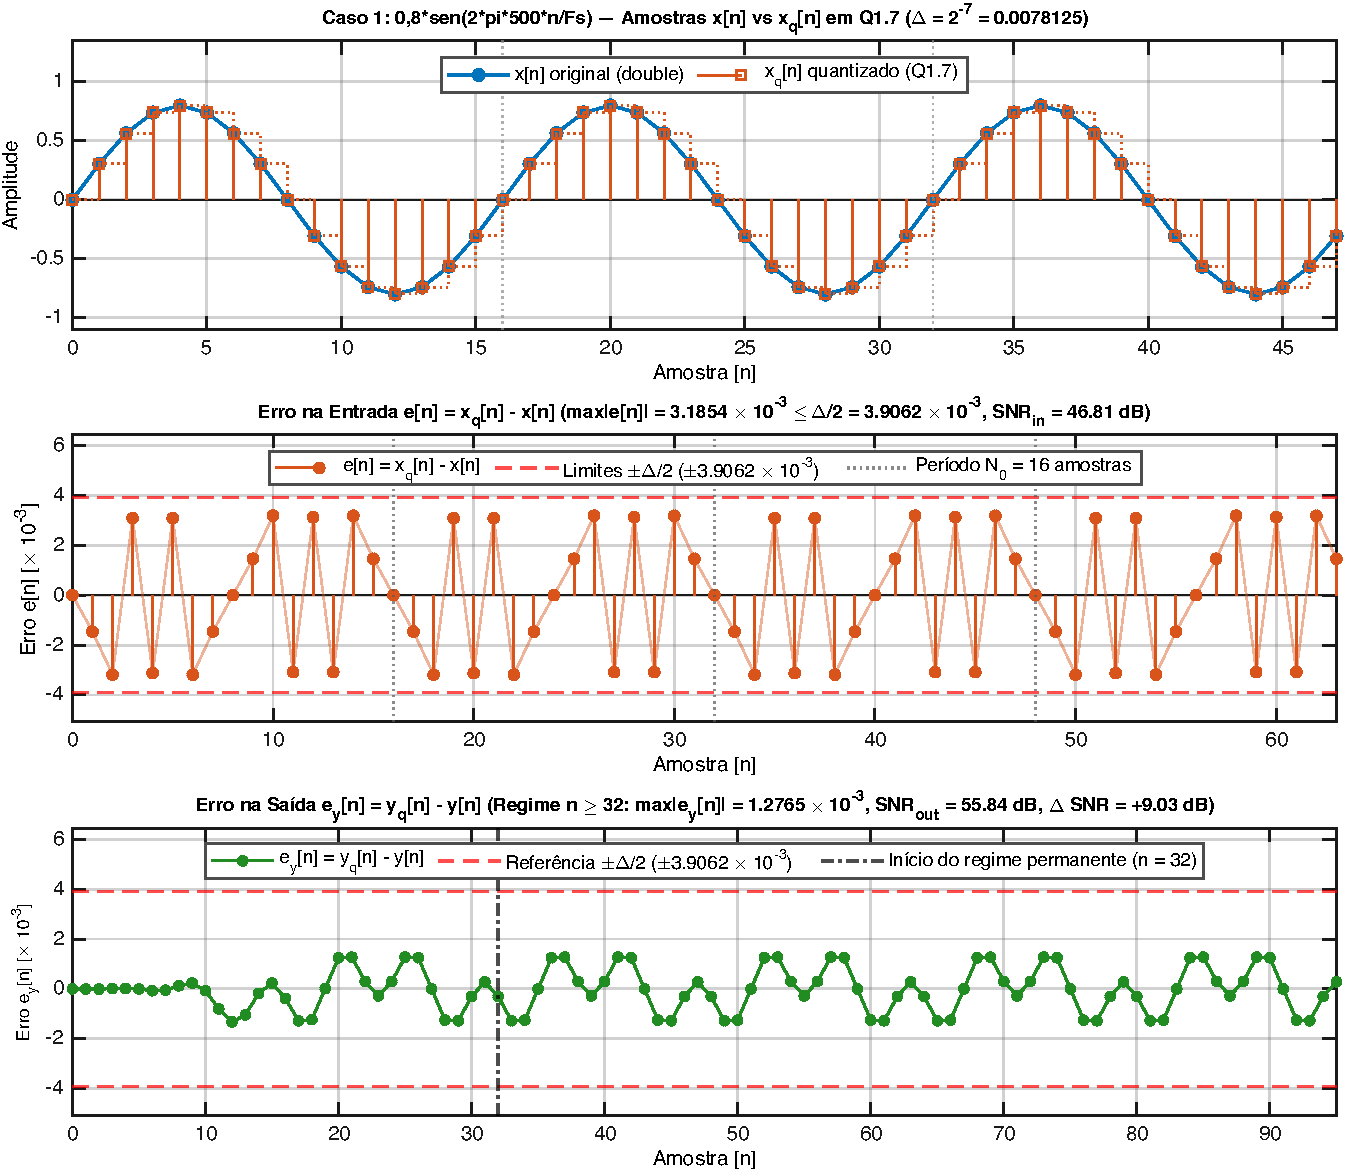
\includegraphics[width=0.92\linewidth, height=0.52\textheight, keepaspectratio]{fig_D1_caso1_amostras_e_erros.pdf}
    \caption{Etapa D (Caso 1 — $\SI{500}{Hz}$): Amostras $x[n]$ e $x_q[n]$ em \texttt{Q1.7} com marcadores discretos, erro periódico $e[n]$ ($N_0=16$) e resíduo filtrado $e_y[n]$.}
    \label{fig:D1_caso1}
\end{figure}

\begin{figure}[!htbp]
    \centering
    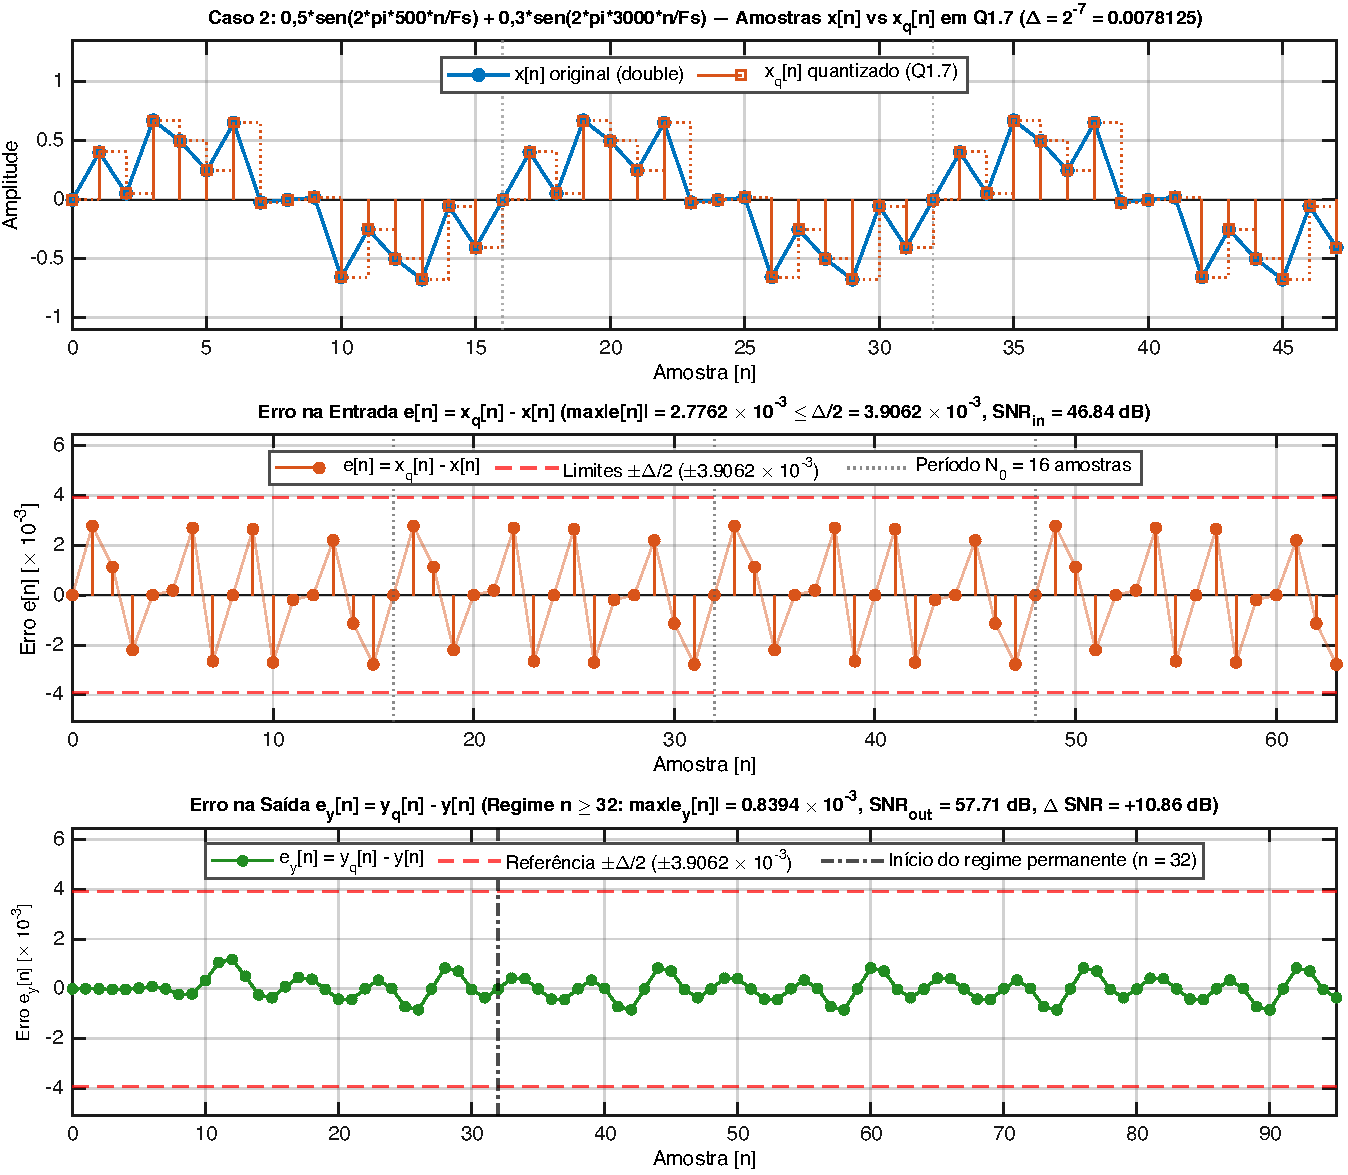
\includegraphics[width=0.92\linewidth, height=0.52\textheight, keepaspectratio]{fig_D2_caso2_amostras_e_erros.pdf}
    \caption{Etapa D (Caso 2 — $\SI{500}{Hz} + \SI{3000}{Hz}$): Amostras $x[n]$ e $x_q[n]$ em \texttt{Q1.7}, erro periódico $e[n]$ ($\le \Delta/2$) e erro atenuado na saída $e_y[n]$.}
    \label{fig:D2_caso2}
\end{figure}

\subsection{Respostas às Questões de Análise (Etapa D)}

\begin{enumerate}[leftmargin=1.5em, itemsep=3pt]
    \item \textbf{Periodicidade de $e[n]$:} \textbf{Sim, período exato $N_0 = 16\text{ amostras}$ ($\SI{2,0}{ms}$)} nos dois casos. Como $500/8000 = 1/16$ e $3000/8000 = 3/8$ têm MMC de período igual a $16$ e $Q(\cdot)$ é determinístico sem memória, $x[n+16]=x[n] \Rightarrow e[n+16]=e[n]$. A concentração do erro em harmônicos ($k\cdot\SI{500}{Hz}$) explica a diferença frente ao modelo branco da Equação~\eqref{eq:sqnr_teorica} ($\SI{47,98}{dB}$ e $\SI{45,23}{dB}$ teóricos vs.\ $\MetricaDCasoISNRIn$ e $\MetricaDCasoIISNRIn\text{ dB}$ medidos).
    \item \textbf{Ação do filtro sobre o erro:} Pela linearidade ($e_y = h * e$), o filtro atenua os harmônicos de distorção situados acima de $\SI{1000}{Hz}$, reduzindo a potência do ruído em $\mathbf{\SI{-9,0463}{dB}}$ (Caso~1) e $\mathbf{\SI{-12,2170}{dB}}$ (Caso~2).
    \item \textbf{Melhora de SNR:} \textbf{Sim, nos dois cenários:} ganho de $\mathbf{\MetricaDCasoIDeltaSNR\text{ dB}}$ no Caso~1 (atingindo $\SI{55,8395}{dB}$) e de $\mathbf{\MetricaDCasoIIDeltaSNR\text{ dB}}$ no Caso~2 (atingindo $\SI{57,7056}{dB}$).
    \item \textbf{Variação conjunta de sinal e ruído:} Pela decomposição logarítmica da variação de SNR,
    \begin{equation}
        \Delta\text{SNR}_{\text{dB}} = 10\log_{10}(P_{y,\text{ss}}/P_x) - 10\log_{10}(P_{e_y,\text{ss}}/P_e) = \Delta P_{\text{sinal,dB}} - \Delta P_{\text{ruído,dB}},
        \label{eq:deltasnr}
    \end{equation}
    no Caso~1 o sinal pertence à passante ($\Delta P_{\text{sinal}} = \SI{-0,0188}{dB}$), logo $\Delta\text{SNR}_1 \approx -\Delta P_{\text{ruído}}$. No Caso~2, a supressão da senoide de $\SI{3000}{Hz}$ reduz a potência do sinal de entrada em $\mathbf{\SI{-1,3542}{dB}}$ ($0,170 \to 0,12446$), de modo que $\Delta\text{SNR}_2 = -1,3542 - (-12,2170) = \SI{+10,8628}{dB}$ reflete conjuntamente a filtragem do sinal e do ruído.
\end{enumerate}

% ==============================================================================
% 8. ETAPA E — PRECISÃO ARITMÉTICA E OVERFLOW
% ==============================================================================
\FloatBarrier
\section{Etapa E — Precisão Aritmética e \textit{Overflow} em Ponto Fixo}

Além da quantização de dados, operações em palavra finita geram erros de reconversão após multiplicações e risco de \textit{overflow}~\cite{aula17}. Multiplicando dois operandos exatos em \texttt{Q1.7} ($a = 79/128 = 0,6171875$ e $b = 45/128 = 0,3515625$):
\begin{equation}
    p_{\text{exato}} = a \cdot b = \frac{3555}{16384} = \MetricaEProdCompleto \quad (\texttt{00.00110111100011}_2\text{ em \texttt{Q2.14}}).
\end{equation}
O retorno de \texttt{Q2.14} ($16\text{ bits}$) para \texttt{Q1.7} ($8\text{ bits}$) descarta $7\text{ LSBs}$ ($99/16384 = 0,7734375\text{ LSB}_{\text{Q1.7}}$). A Tabela~\ref{tab:E1_ponto_fixo} sintetiza o arredondamento, o truncamento, a norma $\ell_1$ e o exemplo de \textit{overflow}.

\begin{table}[!htbp]
    \centering
    \caption{Etapa E: Multiplicação \texttt{Q1.7}$\to$\texttt{Q2.14}$\to$\texttt{Q1.7}, norma $\ell_1$ ($\sum|h[k]|$) e \textit{overflow} em adição \texttt{Q1.7} ($0,75+0,50$).}
    \label{tab:E1_ponto_fixo}
    \scriptsize
    \setlength{\tabcolsep}{4.5pt}
    \renewcommand{\arraystretch}{1.08}
    \begin{adjustbox}{max width=\textwidth}
    \begin{tabular}{@{}lllcrr@{}}
        \toprule
        \textbf{Operação / Grandeza} & \textbf{Formato} & \textbf{Fração} & \textbf{Palavra Binária} & \multicolumn{1}{c}{\textbf{Valor Decimal}} & \multicolumn{1}{c}{\textbf{Erro / Observação}} \\
        \midrule
        Operando $a$ & \texttt{Q1.7} ($8\text{ bits}$) & $79 / 128$ & \texttt{0.1001111} & $+0,61718750000000$ & $0,00000000000000$ \\
        Operando $b$ & \texttt{Q1.7} ($8\text{ bits}$) & $45 / 128$ & \texttt{0.0101101} & $+0,35156250000000$ & $0,00000000000000$ \\
        \textbf{Produto completo ($a \cdot b$)} & \textbf{\texttt{Q2.14} ($16\text{ bits}$)} & $\mathbf{3555 / 16384}$ & \texttt{00.00110111100011} & $\mathbf{+0,21697998046875}$ & $7\text{ LSBs} = 0,7734375\text{ LSB}$ \\
        \rowcolor{rowpass}
        \textbf{Arredondado (\texttt{round})} & \textbf{\texttt{Q1.7} ($8\text{ bits}$)} & $\mathbf{28 / 128}$ & \texttt{0.0011100} & $\mathbf{+0,21875000000000}$ & $\mathbf{+0,00177002}$ ($+0,2266\text{ LSB}$) \\
        \rowcolor{rowfail}
        \textbf{Truncado (\texttt{floor})} & \textbf{\texttt{Q1.7} ($8\text{ bits}$)} & $\mathbf{27 / 128}$ & \texttt{0.0011011} & $\mathbf{+0,21093750000000}$ & $\mathbf{-0,00604248}$ ($-0,7734\text{ LSB}$) \\
        \midrule
        Norma $\ell_1$ ($\sum_{k=0}^{22} |h[k]|$) & \texttt{double} ($N=23$) & --- & --- & $+1,47339547500902$ & $\lceil\log_2(1,4734)\rceil = 1\text{ bit guarda}$ \\
        Soma exata ($0,75 + 0,50$) & \texttt{Q2.7} ($9\text{ bits}$) & $160 / 128$ & \texttt{01.0100000} & $+1,25000000000000$ & Excede $+127/128$ (\textit{Overflow}) \\
        \rowcolor{rowpass}
        Soma com \textbf{Saturação} & \texttt{Q1.7} ($8\text{ bits}$) & $+127 / 128$ & \texttt{0.1111111} & $+0,99218750000000$ & $-0,2578125$ ($-33\text{ LSB}$) \\
        \rowcolor{rowfail}
        Soma com \textbf{\textit{Wrap-Around}} & \texttt{Q1.7} ($8\text{ bits}$) & $-96 / 128$ & \texttt{1.0100000} & $-0,75000000000000$ & $\mathbf{-2,0000000}$ ($\mathbf{-256\text{ \textbf{LSB}}}$) \\
        \bottomrule
    \end{tabular}
    \end{adjustbox}
\end{table}

\begin{enumerate}[leftmargin=1.5em, itemsep=3pt]
    \item \textbf{Crescimento de palavra e acumulador MAC:} O produto \texttt{Q1.7}$\times$\texttt{Q1.7} exige $14\text{ bits}$ fracionários e $2\text{ bits}$ inteiros (\textbf{\texttt{Q2.14}}, $16\text{ bits}$), cobrindo $(-1)\times(-1)=+1$. Ao retornar para \texttt{Q1.7}, o arredondamento limita $|e|\le \Delta/2$ ($+0,2266\text{ LSB}$), enquanto o truncamento impõe viés negativo ($-0,7734\text{ LSB}$, $3,41\times$ maior)~\cite{aula17}. Para somar $N = 23$ parcelas no pior caso algébrico irrestrito, o acumulador demanda $\lceil\log_2(23)\rceil = 5\text{ bits}$ de guarda ($21\text{ bits}$ mínimos)~\cite{lyons2011}.
    \item \textbf{Norma $\ell_1$ ($\sum|h[k]|$) como limite físico:} Para $|x[n]| \le X_{\text{máx}} = 1$, a desigualdade triangular estabelece o supremo BIBO:
    \begin{equation}
        |y[n]| = \left|\sum_{k=0}^{22} h[k]\,x[n-k]\right| \le X_{\text{máx}} \sum_{k=0}^{22} |h[k]| = \MetricaENormaLI \;\; (\MetricaENormaLIdB\text{ dB}),
        \label{eq:l1bound}
    \end{equation}
    exigindo $\lceil\log_2(1,4734)\rceil = \mathbf{1\text{ bit de guarda}}$ específico para este filtro (ou escalonamento prévio por $1/\|h\|_1 \approx 0,6787$).
    \item \textbf{\textit{Overflow}: saturação vs.\ \textit{wrap-around}:} Excedida a faixa $[-1,\, +0,9921875]$ (como em $+0,75 + 0,50 = +1,25$), a \textbf{saturação} limita a saída em $+127/128 = +0,9921875$ mantendo a polaridade, enquanto o \textbf{\textit{wrap-around}} modular em complemento de dois inverte o bit de sinal para $-96/128 = -0,75$ (erro severo de $-2,0$)~\cite{aula17}.
\end{enumerate}

% ==============================================================================
% 9. CONCLUSÃO TÉCNICA (NOS 5 EIXOS EXIGIDOS PELO ROTEIRO)
% ==============================================================================
\FloatBarrier
\section{Conclusão Técnica}

A síntese dos resultados obtidos nos cinco eixos exigidos pelo roteiro~\cite{roteiro2026} demonstra:

\begin{enumerate}[label=\textbf{(\roman*)}, leftmargin=2.1em, itemsep=3.5pt]
    \item \textbf{Projeto e atendimento à máscara:} A estimativa $N_{\text{est}} = 22$ mostrou-se insuficiente ($N=21, 22$ reprovam em $\SI{2200}{Hz}$ com $40,61$ e $\SI{44,06}{dB} < \SI{45}{dB}$), sendo $\mathbf{N = 23}$ ($M = 22$, Tipo~I) o menor comprimento aprovado com janela de Hamming ($\delta_{p,\text{máx}} = \SI{0,042323}{dB}$, $A_{s,\text{mín}} = \SI{47,0065}{dB}$, ganho DC $= \SI{0}{dB}$ e $\tau_g = \SI{11,0}{amostras} = \SI{1,3750}{ms}$). O projeto ótimo \textit{Equiripple} cumpriu a mesma máscara com $N_{\text{eq}} = 15$, reduzindo em $\MetricaAIIReducaoCoefsPerc\%$ os MACs/s e em $36,36\%$ a latência ($\SI{7,0}{amostras}$).

    \item \textbf{Correção funcional do buffer circular:} A rotina \texttt{fir\_circular(x, h)} operou em $O(1)$ sem cópias de memória, reproduzindo \texttt{filter(h,1,x)} com erro nulo no impulso e precisão de máquina nas senoides ($\MetricaBErroMaxSenFilter$), com ganhos espectrais confirmados via \texttt{freqz} ($\MetricaBGanhoPassdB\text{ dB}$ em $\SI{500}{Hz}$ e $\MetricaBGanhoStopdB\text{ dB}$ em $\SI{3000}{Hz}$).

    \item \textbf{Efeitos da quantização de coeficientes:} Ambos os formatos preservaram a simetria par, a fase linear Tipo~I e a estabilidade BIBO. Enquanto \textbf{\texttt{Q1.15}} manteve folga na máscara ($\delta_{p,\text{máx}} = \SI{0,042440}{dB}$, $A_{s,\text{mín}} = \SI{46,9752}{dB}$), \textbf{\texttt{Q1.7}} anulou $k=0,22$, reduziu a rejeição para $\SI{39,8632}{dB}$ e deslocou o ganho DC para $\SI{-0,205999}{dB}$ ($\sum h_Q = 125/128$), reprovando nas duas bandas.

    \item \textbf{Efeitos da quantização de amostras:} Em \texttt{Q1.7}, o erro de entrada manteve-se contido em $\pm\Delta/2$ com período exato de $16\text{ amostras}$. A filtragem passa-baixa atenuou os harmônicos de alta frequência do ruído e elevou a SNR pós-transitório ($n\ge 32$) em $\MetricaDCasoIDeltaSNR\text{ dB}$ (Caso~1) e $\MetricaDCasoIIDeltaSNR\text{ dB}$ (Caso~2), evidenciando via $\Delta\text{SNR} = \Delta P_{\text{sinal}} - \Delta P_{\text{ruído}}$ o efeito conjunto da supressão de $\SI{3000}{Hz}$ ($\Delta P_{\text{sinal}} = \SI{-1,3542}{dB}$ no Caso~2).

    \item \textbf{Limites da aritmética finita:} A multiplicação \texttt{Q1.7}$\times$\texttt{Q1.7} exige palavra intermediária \texttt{Q2.14} ($16\text{ bits}$), sendo o arredondamento $3,41\times$ mais exato que o truncamento no exemplo testado. A norma $\|h\|_1 = \MetricaENormaLI$ requer ao menos $1\text{ bit}$ de guarda no acumulador ($5\text{ bits}$ no caso irrestrito $N=23$) e aritmética saturada contra \textit{wrap-around}.
\end{enumerate}

% ==============================================================================
% 10. REFERÊNCIAS BIBLIOGRÁFICAS (SEMPRE EM PÁGINA SEPARADA)
% ==============================================================================
\clearpage
\begingroup
\small
\begin{thebibliography}{99}\setlength{\itemsep}{3pt}\setlength{\parskip}{0pt}

\bibitem{roteiro2026}
SARNO FILHO, Elio Pithon. \textit{Roteiro da Prática 3: Projeto de Filtro FIR Passa-Baixa}. Processamento Digital de Sinais (GRD-MEE-0072), Curso de Engenharia Elétrica, Centro Universitário SENAI CIMATEC, Salvador, 2026.

\bibitem{aula12}
SARNO FILHO, Elio Pithon. \textit{Aula 12 --- Filtros Digitais}. Notas de aula de Processamento Digital de Sinais (GRD-MEE-0072), Curso de Engenharia Elétrica, Centro Universitário SENAI CIMATEC, Salvador, 2026.

\bibitem{aula13}
SARNO FILHO, Elio Pithon. \textit{Aula 13 --- Filtros FIR de Fase Linear}. Notas de aula de Processamento Digital de Sinais (GRD-MEE-0072), Curso de Engenharia Elétrica, Centro Universitário SENAI CIMATEC, Salvador, 2026.

\bibitem{aula14}
SARNO FILHO, Elio Pithon. \textit{Aula 14 --- Filtros FIR de Fase Linear (Parte 2)}. Notas de aula de Processamento Digital de Sinais (GRD-MEE-0072), Curso de Engenharia Elétrica, Centro Universitário SENAI CIMATEC, Salvador, 2026.

\bibitem{aula15}
SARNO FILHO, Elio Pithon. \textit{Aula 15 --- Filtros FIR de Fase Linear (Parte 3)}. Notas de aula de Processamento Digital de Sinais (GRD-MEE-0072), Curso de Engenharia Elétrica, Centro Universitário SENAI CIMATEC, Salvador, 2026.

\bibitem{aula16}
SARNO FILHO, Elio Pithon. \textit{Aula 16 --- Implementação FIR}. Notas de aula de Processamento Digital de Sinais (GRD-MEE-0072), Curso de Engenharia Elétrica, Centro Universitário SENAI CIMATEC, Salvador, 2026.

\bibitem{aula17}
SARNO FILHO, Elio Pithon. \textit{Aula 17 --- Quantização em Filtros FIR (Parte 1)}. Notas de aula de Processamento Digital de Sinais (GRD-MEE-0072), Curso de Engenharia Elétrica, Centro Universitário SENAI CIMATEC, Salvador, 2026.

\bibitem{diniz2014}
DINIZ, Paulo S. R.; DA SILVA, Eduardo A. B.; NETTO, Sergio L. \textit{Processamento Digital de Sinais: Projeto e Análise de Sistemas}. 2. ed. Porto Alegre: Bookman, 2014.

\bibitem{oppenheim2010}
OPPENHEIM, Alan V.; SCHAFER, Ronald W. \textit{Discrete-Time Signal Processing}. 3. ed. Upper Saddle River: Pearson, 2010.

\bibitem{lyons2011}
LYONS, Richard G. \textit{Understanding Digital Signal Processing}. 3. ed. Boston: Prentice Hall, 2011.

\bibitem{manolakis2011}
MANOLAKIS, Dimitris G.; INGLE, Vinay K. \textit{Applied Digital Signal Processing: Theory and Practice}. Cambridge: Cambridge University Press, 2011.

\bibitem{mathworks2026}
THE MATHWORKS, INC. \textit{Signal Processing Toolbox: User's Guide (\texttt{firpm}, \texttt{firpmord}, \texttt{freqz} e Filter Designer)}. Natick: MathWorks, R2026b.

\end{thebibliography}
\endgroup

\end{document}
